\chapter{Propuesta solución: Aplicación Aprende Fácil}
\label{cap:aprendeFacil}

\setcounter{secnumdepth}{5} % para que ponga 1.1.1.1 en subsubsecciones
\setcounter{tocdepth}{5}

%-------------------------------------------------------------------
\section{Diseño de la Aplicación}
%-------------------------------------------------------------------
\label{cap:sec:disenioInterfaz}
Como ya se ha explicado en capítulos anteriores, esta aplicación está creada por y para personas que tienen alguna discapacidad cognitiva, por lo que el diseño de la interfaz debe ser sencillo y su uso no debe llevar a confusión ni debe hacer sentir al usuario frustrado al usarla. 
Es por ello que el diseño debe estar centrado en el usuario, y en nuestro caso aún más puesto que los usuarios finales requieren un diseño centrado en sus necesidades. Así pues, al ser un campo poco conocido por lo integrantes del equipo, se ha necesitado de la ayuda de expertos para saber con mas detalle cual es el diseño adecuado. 
El diseño de la aplicación se ha realizado en dos iteraciones: una iteración competitiva entre los integrantes del grupo y una segunda iteración con expertos del Colegio Estudio3 Afanias\footnote{https://afanias.org/que-hacemos/educacion/colegio-estudio-3/}. 

%-------------------------------------------------------------------

\subsection{Primera Iteración: Iteración Competitiva}
%-------------------------------------------------------------------
\label{cap:subsec:iteracionCompetitiva}

En esta primera iteración cada integrante del grupo ha realizado su propio diseño de la aplicación. En la realización de estos diseños, los integrantes no podían hablar entre ellos ni comentar las diferentes ideas que tenían para la implementación. De esta forma se consigue que los diseños sean totalmente dispares y que las ideas de uno no provoquen la modificación del diseño del otro y que surjan ideas distintas.
Se realizaron cuatro prototipos distintos ya que no teníamos claro si los usuarios finales iban a preferir que se mostrara un solo significado o todos, si mostrar la definición y el ejemplo les iba a ayudar o no y si añadir los pictogramas les ayudaría o no.
Los prototipos fueron los siguientes:
\begin{itemize}
	\item Prototipo 1: Se muestra un único significado, siendo este el más común e incluyendo las comparaciones.
	\item Prototipo 2: Se muestra el significado más común, junto con una definición tradicional del concepto e incluyendo las comparaciones.
	\item Prototipo 3: Se muestran todos los significados de la palabra buscada e incluyendo las comparaciones.
	\item Prototipo 4: Se muestran todos los significados de la palabra y se añaden pictogramas\footnote{Se entiende como pictograma un dibujo, imagen o figura que representa el significado de una palabra.} a las palabras, haciendo así que la comprensión del concepto sea mucho mas sencilla. Tanto en el prototipo diseñado por Pablo como en el de Irene se han utilizado los pictogramas de ARASAAC\footnote{http://www.arasaac.org/}.
	
\end{itemize}

En las Figuras \ref{fig:mockup1pablo}, \ref{fig:mockup2pablo}, \ref{fig:mockup3pablo} y \ref{fig:mockup4pablo} se muestran los prototipos creados por Pablo y en las Figuras \ref{fig:mockup1irene_vInicial}, \ref{fig:mockup2irene_vInicial},  \ref{fig:mockup3irene_vInicial} y \ref{fig:mockup4irene_vInicial} los prototipos creados por Irene.

Una vez que los prototipos estaban terminados, lnos juntamos para hacer una puesta en común y analizar los prototipos creados. 
Por lo general, los prototipos de los dos integrantes del grupo eran bastantes similares, las principales diferencias eran:

\begin{itemize}
	\item Ambos prototipos integran los mismos elementos: un campo de texto para introducir la palabra, un botón de búsqueda y los resultados se muestran en forma de lista, agrupando los distintos resultados en rectángulos, que a partir de ahora denominaremos fichas.
	Pablo ha optado por formas rectangulares, tanto para las fichas como para el campo de texto, mientras que Irene utiliza formas redondeadas en todos los elementos. 
	Por otro lado, Pablo implementó un diseño orientado a niños por lo que para el color utilizó azules muy suaves y fondos juveniles con lápices de colores, gomas de borrar, etc.  Irene utilizó un color mostaza, siendo un diseño más simple pero intentando abarcar a un usuario de cualquier edad. Por último, los resultados del prototipo de Irene, se muestran en color mostaza indicando de esta forma que se pueden pinchar en ellos, y se realizará la búsqueda del concepto pulsado.
	
	\item El orden a la hora de mostrar los resultados es distinto. En los prototipos de Pablo se muestran primero las metáforas (\textit{Un vehículo es una máquina} o \textit{Un vehículo es un transporte}), después los símiles (\textit{Un vehículo es como un taxi}) y finalmente las analogías (\textit{Un vehículo es rápido como un caballo}). En los prototipos de Irene se muestra únicamente una analogía, una metáfora y un símil para cada significado de la palabra buscada.
	
	\item En el prototipo 3 de Pablo incluye justo debajo de los resultados mostrados un ejemplo siempre visible (``Él necesita un coche para ir a trabajar'') para facilitar al usuario la comprensión del término buscado.
	
	 \item En el prototipo 3 de Irene incluye justo debajo de los resultados mostrados una definición dentro de un botón (``Vehículo motorizado de cuatro ruedas por lo general impulsado por un motor de combustión interna'') dando a elegir al usuario la decisión de poder verla o no.
	
	\item Pablo decidió añadir el título ``Un X es ...'' antes de la lista de los resultados, englobando de esta forma los conceptos que tienen el mismo significado. Si existen varias acepciones del concepto, añade el título ``O también puede ser...'' en los siguientes, dejando claramente divididos los distintos significados que pudieran existir para el concepto buscado. En cambio Irene, añade un único título al principio (``Resultados para la palabra X'') donde queda claro que los resultados que se obtienen son para dicho concepto y además añade delante de cada metáfora: ``Un X es...''  y delante de cada símil y analogía: ``Un X es como...''.

	\item Para la numeración de los resultados obtenidos, Pablo incluye dentro de cada ficha un listado numérico e Irene únicamente añade un número a la ficha.
	
	\item En el prototipo donde se incluyen también los pictogramas, Pablo añade un pictograma que hace referencia al concepto buscado según el contexto en que se utilice. Por ejemplo, un vehículo puede hacer referencia a un coche o puede ser un medio para llegar o lograr un fin, por lo que el añade el pictograma en función de su significado, e Irene además de incluir el mismo pictograma que Pablo, añade pictogramas a las palabras usadas en las comparaciones. Por ejemplo, en la frase ``Un portero es un vigilante'' Irene añadió el pictograma de vigilante.
\end{itemize}



Una vez analizados los prototipos de ambos integrantes nos reunimos con los directores del trabajo y se decidió crear un prototipo con las siguientes características:


\begin{itemize}
	\item Para el diseño de la interfaz se eligió el de Irene por tener una interfaz más atractiva.
	\item Se eligió la palabra Portero para utilizarla como ejemplo en todos los prototipos.
	\item El orden de las resultados se modificó, haciendo que primero aparezcan las metáforas (``Un portero es un vigilante''), después los símiles (``Un portero es como un guardia'') y por último las analogías  (``Un portero es tan ágil como un pájaro'').
	\item Se eliminó la palabra \textit{tan} en la plantilla usada para las analogías.
	\item Se creó un nombre para la aplicación que estuviese en español: ``Aprende Fácil''.
	\item En vez de mostrar un único símil, una metáfora y una analogía. Se deben mostrar todos los resultados obtenidos para dicho concepto.
	\item Se decidió que si la palabra solo tenía un significado se eliminaba el número de la ficha.
	\item Se añadió un pictograma a la característica que relaciona el concepto con el resultado en las analogías. Por ejemplo, en la frase \textit{Un portero es tan fuerte como un gorila}  se añadió el pictograma correspondiente a fuerte.
	\item Dejar el ejemplo del prototipo de Pablo junto con la definición del prototipo de Irene.
	\item Crear un nuevo prototipo donde la definición y el ejemplo se muestren a primera vista, y el usuario no tenga que estar pinchando en ningún botón para que los expertos nos indiquen cual es la mejor opción.
	\item Crear otro prototipo donde la definición y el ejemplo estén separados. Así el usuario puede elegir lo que quiere ver, si solo una cosa o ambas.
\end{itemize} 

Con todas estas decisiones, se crearon los prototipos que se muestran en las Figuras \ref{fig:mockup1irene_vFinal}, \ref{fig:mockup2irene_v1_vFinal}, \ref{fig:mockup2irene_v2_vFinal}, \ref{fig:mockup2irene_v3_vFinal}, \ref{fig:mockup3irene_vFinal}, \ref{fig:mockup4irene_vFinal} y que fueron los que se usaron para en la siguiente iteración donde nos reunimos con los expertos para que nos dieran su opinión sobre la aplicación, y nos ayudarán a decidir sobre los siguientes aspectos:
\begin{itemize}
	\item ¿Se debe mostrar el significado más común o todos los significados de la palabra buscada?
	\item ¿Se debe añadir la definición tradicional y el ejemplo junto con las figuras retóricas o no?  Y en caso de añadirlos, ¿Se deben mostrar juntos en un mismo botón, en distintos botones o sin botón y que aparezcan debajo de los resultados?
	\item ¿Son útiles los pictogramas? En caso de serlo, ¿solamente el pictograma de la palabra buscada o también añadimos los pictogramas de las palabras que se usan en las figuras retóricas?
	\item ¿La forma de mostrar los resultados es correcta, o es mejor otra disposición?
	
\end{itemize} 


 	\figura{Bitmap/Mockups/mockup1_pablo}{width=1.0\textwidth}{fig:mockup1pablo}{Prototipo de Pablo mostrando resultado más común para la palabra vehículo}
	\figura{Bitmap/Mockups/mockup2_pablo}{width=.9\textwidth}{fig:mockup2pablo}{Prototipo de Pablo mostrando resultado más común para la palabra vehículo y un ejemplo} 
	\figura{Bitmap/Mockups/mockup3_pablo}{width=.9\textwidth}{fig:mockup3pablo}{Prototipo de Pablo mostrando todos los resultados para la palabra vehículo} 
 	\figura{Bitmap/Mockups/mockup4_pablo}{width=.9\textwidth}{fig:mockup4pablo}{Prototipo de Pablo mostrando todos los resultados para la palabra vehículo junto con pictogramas} 
 	
 	\figura{Bitmap/Mockups/mockup1_irene_inicial.png}{width=1.2\textwidth}{fig:mockup1irene_vInicial}{Prototipo de Irene mostrando resultado más común para la palabra vehículo}
 	\figura{Bitmap/Mockups/mockup2_irene_inicial.png}{width=1.2\textwidth}{fig:mockup2irene_vInicial}{Prototipo de Irene mostrando resultado más común para la palabra vehículo y una definición}
	\figura{Bitmap/Mockups/mockup3_irene_inicial.png}{width=1.2\textwidth}{fig:mockup3irene_vInicial}{Prototipo de Irene mostrando todos los resultados para la palabra portero} 
	\figura{Bitmap/Mockups/mockup4_irene_inicial.png}{width=1.2\textwidth}{fig:mockup4irene_vInicial}{Prototipo de Irene mostrando todos los resultados para la palabra portero junto con pictogramas} 
	
	\figura{Bitmap/Mockups/mockup1_irene_final.png}{width=1.2\textwidth}{fig:mockup1irene_vFinal}{Prototipo mostrando resultado más común para la palabra portero}
	\figura{Bitmap/Mockups/mockup2_irene_final_v1.png}{width=1.2\textwidth}{fig:mockup2irene_v1_vFinal}{Prototipo Versión 1 mostrando resultado más común para la palabra portero junto con una definición y un ejemplo separados}
	\figura{Bitmap/Mockups/mockup2_irene_final_v2.png}{width=1.2\textwidth}{fig:mockup2irene_v2_vFinal}{Prototipo Versión 2 mostrando resultado más común para la palabra portero junto con una definición y un ejemplo a simple vista}
	\figura{Bitmap/Mockups/mockup2_irene_final_v3.png}{width=1.2\textwidth}{fig:mockup2irene_v3_vFinal}{Prototipo Versión 3 mostrando resultado más común para la palabra portero junto con una definición y un ejemplo en un mismo botón}
	\figura{Bitmap/Mockups/mockup3_irene_final.png}{width=1.2\textwidth}{fig:mockup3irene_vFinal}{Prototipo mostrando todos los resultados para la palabra portero}
	\figura{Bitmap/Mockups/mockup4_irene_final.png}{width=1.2\textwidth}{fig:mockup4irene_vFinal}{Prototipo mostrando todos los resultados para la palabra portero incluyendo los pictogramas}

	
	 
%-------------------------------------------------------------------
\subsection{Segunda Iteración: Evaluación con Expertos}
%-------------------------------------------------------------------
\label{cap:subsec:evaluacionExpertos}

El día 26 de Marzo de 2019 a las 09:00h nos reunimos con la directora y los profesores del colegio Estudio3 Afanias\footnote{https://afanias.org/que-hacemos/educacion/colegio-estudio-3/} situado en la Comunidad de Madrid. Este colegio atiende a niños y jóvenes con discapacidad intelectual entre los 3 y 21 años de edad.

Lo primero que hicimos fue presentarles la aplicación y mostrarles los prototipos creados al final de la iteración anterior (Figuras \ref{fig:mockup1irene_vFinal}, \ref{fig:mockup2irene_v1_vFinal}, \ref{fig:mockup2irene_v2_vFinal}, \ref{fig:mockup2irene_v3_vFinal}, \ref{fig:mockup3irene_vFinal}, \ref{fig:mockup4irene_vFinal}).
Una vez expuestos los distintos prototipos, nos dieron la enhorabuena y nos hicieron participes de la gran ayuda que supondría esta herramienta. A continuación nos dieron su opinión sobre distintos aspectos que se podrían mejorar:

\begin{itemize} 
	\item Modificar el color amarillo-mostaza de los textos por un color más oscuro que contraste más con el fondo blanco. El color actual es morado oscuro para la barra que contiene el título de la aplicación y un violeta para resaltar los resultados obtenidos, así como para el botón de Definición y Ejemplo.
	\item El tipo de letra debe ser Arial o Script, ya que son las letras con las que los alumnos están familiarizados y las que mejor entienden.
	\item Añadir un reproductor que lea la frase, para hacer la aplicación accesible a aquellas personas que no puedan leer.
	\item Incluir la opción de poder ver un video para complementar la información devuelta por la aplicación.
	\item Los pictogramas deben situarse debajo de la palabra y no al lado, ya que los expertos comentaron que esto puede llevar a confusión a los alumnos pensando que sería otra palabra más para leer. 
	\item Introducción de distintas personalizaciones:
	\begin{itemize}
		\item Búsqueda en tres niveles: sencillo, medio y amplio. El nivel sencillo sería realizando la búsqueda de las palabras fáciles en las 1.000 palabras más usadas de la RAE, el medio en las 5.000 palabras más usadas de la RAE y el amplio en las 10.000 palabras más usadas de la RAE. 
		\item Añadir una opción que permita poner todos los textos en mayúsculas, haciendo la aplicación más accesible para aquellos alumnos que no entienden los textos en minúsculas.
		\item Dejar que el usuario configure si quiere que aparezca la definición y el ejemplo o no.
		\item Dejar que el usuario configure  si aparecen los pictogramas o no.
	\end{itemize}
\end{itemize}

Teniendo en cuenta las observaciones de los expertos se creo el diseño final de la aplicación.





%-------------------------------------------------------------------
\section{Implementación de la Aplicación}
%-------------------------------------------------------------------
%-------------------------------------------------------------------
\subsection{Arquitectura de Aprende Fácil}
%-------------------------------------------------------------------
En este apartado se describirá la arquitectura diseñada para la aplicación. En la Figura \ref{fig:diagrama_arquitectura} se puede ver los distintos componentes por los que está formada.

\begin{figure}[!h]
	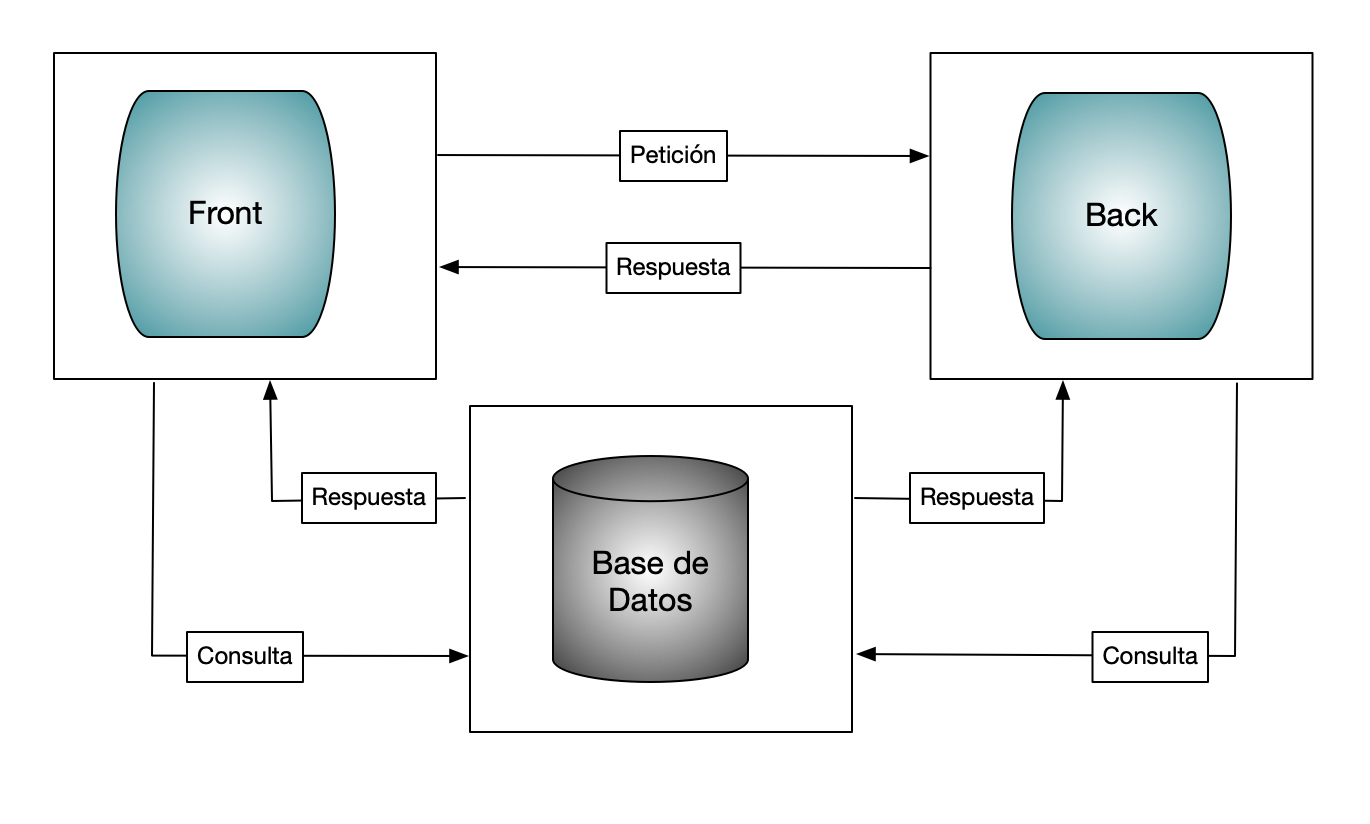
\includegraphics[width=.9\textwidth]{Imagenes/Bitmap/Capitulo4/DiagramaArquitectura.png}
	\caption{Diagrama de la arquitectura del proyecto}
	\label{fig:diagrama_arquitectura}
\end{figure}

La aplicación está formada por una interfaz (\textit{frontend}) la cuál realiza peticiones a la parte interna (\textit{backend}), y este le devuelve la información correspondiente. Para ello, la parte \textit{backend} debe realizar consultas a la base de datos. En la Figura \ref{fig:relacionBackFront}  se puede ver la relación que existe entre el \textit{frontend} con el \textit{backend}, y los servicios web que son utilizados para la obtención de los resultados.
Si el usuario introduce una palabra, dejando por defecto las distintas opciones que vienen y realiza la búsqueda de un concepto, la aplicación invocará a los servicios web relacionados con la obtención de metáforas (\textit{getMetaphor}) y símiles (\textit{getSimil}). A parte, si el usuario seleccionara la opción de ``Mostrar definición y ejemplo'', el servicio web invocado sería el \textit{getDefAndExample} y en caso de seleccionar la opción  ``Mostrar pictos'' se invocaría al servicio web ``getImagen'' para obtener el pictograma del resultado principal y ``getImagenPalabra'' para obtener el pictograma de cada resultado mostrado.

\begin{figure}[!h]
	\includegraphics[width=1.2\textwidth]{Imagenes/Bitmap/Capitulo4/RelacionBackFront.png}
	\caption{Relación entre \textit{Backend} y \textit{Frontend}}
	\label{fig:relacionBackFront}
\end{figure}


 Igualmente en los siguientes apartados se explicará con mayor detalle tanto la implementación del \textit{frontend} como del \textit{backend} . 

Por último, la Universidad Complutense de Madrid nos facilitó un contenedor para poder alojar nuestro trabajo, accesible en la dirección \textit{holstein.fdi.ucm.es}. Este servidor no tenía instalado ningún servicio por lo que se tuvo que realizar la instalación de todo lo necesario (python, pyp, git, mysql, etc). Una vez clonada la rama de GitHub donde tenemos el proyecto, el siguiente paso fue dejar el servidor siempre activo, para ello se tuvo que crear un servicio (\textit{.service}) donde se guardaría la ruta del proyecto.

%-------------------------------------------------------------------
\subsection{Base de datos de Aprende Fácil}
%-------------------------------------------------------------------

Para este proyecto, se ha utilizado una base de datos para la persistencia de los datos. El sistema encargado de la gestión de la base de datos corresponde con MariaDB y esta constituida por las tablas que se pueden ver en la Figura \ref{fig:tablasBBDD} :

\begin{figure}[!h]
	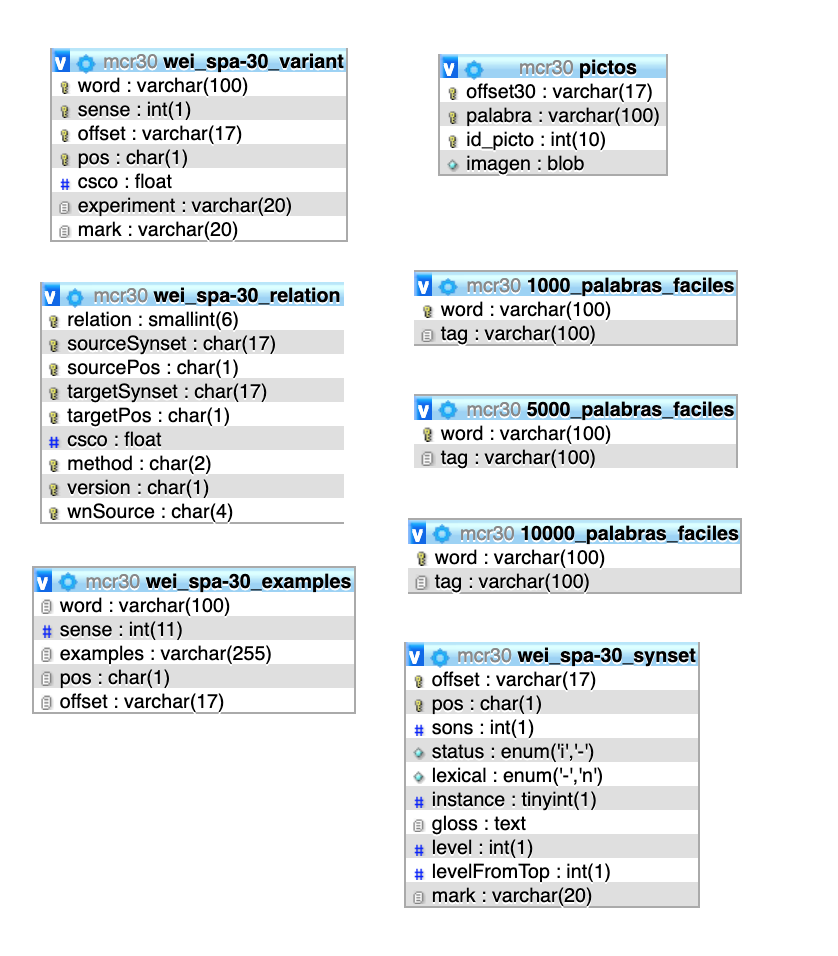
\includegraphics[width=.9\textwidth]{Imagenes/Bitmap/Capitulo4/tablasBBDD.png}
	\caption{Tablas utilizadas en la Base de Datos}
	\label{fig:tablasBBDD}
\end{figure}

\begin{itemize}
	\item Se ha hecho uso de la base de datos propia de WordNet, llamada MCR (\textit{Multilingual Central Repository})\footnote{http://adimen.si.ehu.es/web/MCR/}, y se ha utilizado la versión 3.0.  MCR es una base de datos de código abierto que integra distintas versiones de WordNet para seis lenguajes diferentes: Inglés, Español, Catalán, Vasco, Gallego y Portugués.  
	
	Se han utilizado principalmente cuatro tablas: ``wei\_spa-30\_variant'', ``wei\_spa-30\_relation'', ``wei\_spa-30\_examples'' y ``wei\_spa-30\_synset''. 
	De la tabla ``wei\_spa-30\_variant'' solamente se han utilizado estos atributos:
	\begin{itemize}
		\item \textit{word}: Contiene la palabra. Cuando el usuario introduce la palabra en la aplicación, se realiza una búsqueda en dicha tabla para saber si la palabra buscada se encuentra .
		\item \textit{offset}: Es el identificador de la palabra, aunque una misma palabra puede tener distintos \textit{offsets} (uno por cada acepción). 
	\end{itemize}

	De la tabla ``wei\_spa-30\_relation'', solamente se han utilizado estos atributos:
	\begin{itemize}
		\item \textit{sourceSynset}: Contiene el \textit{offset} de hipónimo.  
		\item \textit{targetSynset}: Contiene el \textit{offset} de hiperónimo.  
	\end{itemize}


	De la tabla ``wei\_spa-30\_examples'', se han utilizado los siguientes atributos:
		\begin{itemize}
		\item \textit{offset}: Contiene el \textit{offset} de la palabra.  
		\item \textit{examples}: Contiene el ejemplo correspondiente.
	\end{itemize}
	
	De la tabla ``wei\_spa-30\_synset'', se han utilizado los siguientes atributos:
	\begin{itemize}
		\item \textit{offset}: Contiene el \textit{offset} de la palabra.  
		\item \textit{gloss}: Contiene la definición correspondiente.
	\end{itemize} 


	\item En vez de tener tres ficheros donde guardar las 1.000, 5.000 y 10.000 palabras más usadas de la RAE, se guardaron los datos en tres tablas llamadas ``1000\_palabras\_faciles'', ``5000\_palabras\_faciles'' y ``10000\_palabras\_faciles''. Las tres se componen de dos columnas:
	\begin{itemize}
		\item \textit{word}: Contiene la palabra fácil.  
		\item \textit{tag}: Contiene el tipo de palabra que es (sustantivo, adjetivo o verbo).
	\end{itemize} 
	 
	 
	\item Una tabla llamada ``pictos'', que almacena la información de los pictogramas y está formada por las siguientes columnas:
	\begin{itemize}
		\item \textit{offset30}: Es el identificador del \textit{synset} en la versión 3.0 de WordNet.
		\item palabra: Contiene la palabra del pictograma.
		\item id\_picto: Es el identificador del pictograma.
		\item imagen: Contiene el pictograma con una codificación binaria ``base64''.
	\end{itemize}

\end{itemize}


%-------------------------------------------------------------------
\subsection{Backend de Aprende Fácil}
%-------------------------------------------------------------------

%-------------------------------------------------------------------
\subsubsection{Selección de la Red Semántica a utilizar}
%-------------------------------------------------------------------
\label{cap:subsec:redsemanticautilizada}

En este trabajo necesitamos una herramienta que nos proporcione las palabras relacionadas con un concepto dado y para ello vamos a emplear una red semántica.
Como se ha comentado en el capítulo 2 existen varias redes semánticas que facilitan sinónimos, términos relacionados, metáforas, hiperónimos, etc. de un concepto dado. 
De todas las posibilidades presentadas en la sección 2.1 solo hay dos redes semánticas disponibles para el castellano: WordNet y ConcepNet. Para decidir con cual de las dos quedarnos hicimos una evaluación de ambas para evaluar si los conceptos devueltos por cada herramienta son correctos y sirven para nuestro propósito. En la sección 4.4.1.1 se explicará el diseño de la prueba que se ha realizado para ver que red semántica se utilizará finalmente en el proyecto, en la sección 5.2 se analizarán los resultados cuantitativos de la prueba realizada, en el punto 5.3, se analizarán los resultados obtenidos a nivel cualitativo y en el 5.4 se describirán las conclusiones finales de la evaluación. Por otra parte, en los apartados posteriores, se detallarán los distintos servicios web utilizados para este proyecto, en la sección 5.5 se hablará de la base de datos utilizada y de su estructura, en los apartados 5.6, 5.7 y 5.8 se describirán los servicios web que se utilizan para la obtención de sinónimos, hipónimos e hiperónimos fáciles respectivamente. Por último, se hablará en los puntos 5.9 y 5.10 sobre los servicios web utilizados para crear las metáforas y los símiles que finalmente leerá el usuario.


%-------------------------------------------------------------------
\subsubsection{Diseño de la evaluación}
%-------------------------------------------------------------------
\label{cap:subsec:disenioeval}


Para decidir que red semántica se iba a usar se decidió hacer una prueba con palabras que fuesen lo más heterogéneas posible, para ello se eligieron tres artículos periodísticos de distintos temas: tecnológico\footnote{https://elpais.com/elpais/2019/04/12/ciencia/1555061040\_073105.html}, deportivo\footnote{https://elpais.com/deportes/2019/04/22/actualidad/1555956020\_022201.html} y político\footnote{https://elpais.com/politica/2019/04/23/actualidad/1556019953\_831941.html}. (Los artículos se pueden ver en el Apéndice \ref{sec:apendiceA} )De los artículos se seleccionaron únicamente los verbos, sustantivos y adjetivos, eliminando las palabras que estuvieran repetidas. Finalmente, quedaron 793 palabras para la realización de la prueba, para cada una de estas palabras se obtuvieron en WordNet y ConceptNet sus sinónimos y términos relacionados (en WordNet se entiende como término relacionado a los hiperónimos e hipónimos).

A continuación se comprobó de manera independiente cuantos de los sinónimos y términos relacionados se encontraban en cada una de las tres listas de palabras fáciles\footnote{listas de 1.000, 5.000 y 10.000 palabras más utilizadas en castellano según la RAE} (análisis cuantitativo). Eligiendo como parámetros: porcentaje de palabras introducidas que no generan ningún resultado, porcentaje de palabras sin términos relacionados, porcentaje de palabras sin sinónimos  y cantidad de palabras generadas por cada red semántica(WordNet y ConceptNet). Por último, se analizó la calidad de las palabras obtenidas por cada una de las redes semánticas en cada una de las listas de palabras fáciles, es decir, si las palabras que generaban tenían una relación aceptable con la palabra origen (análisis cualitativo). Eligiendo en ese caso como parámetros el porcentaje de sinónimos correctos y el porcentaje de términos relacionados correctos.

%-------------------------------------------------------------------
\subsubsection{Resultados cuantitativos}
%-------------------------------------------------------------------
\label{cap:sec:pruebaCuantitativa}
\begin{figure}[!h]
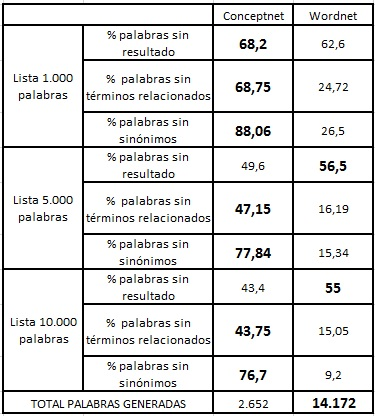
\includegraphics[width=1.0\textwidth]{Imagenes/Bitmap/Capitulo4/tabla_cuantitativa}
\caption{Tabla de resultados de la prueba cuantitativa}
\label{fig:tabla_cuantitativa}
\end{figure}

En la Tabla \ref{fig:tabla_cuantitativa} se muestran los resultados de la prueba cuantitativa realizada, como se puede observar, en términos generales, WordNet ofrece mejores resultados que ConceptNet ya que el porcentaje de palabras sin términos relacionados, sinónimos o ambas, es mayor en esta última. En el caso de la primera lista utilizada (1.000 palabras fáciles) ConceptNet no encontró ningún resultado para el 68,2\% de las palabras introducidas mientras que WordNet no encontró nada para el 62,6\%. En el caso de los términos relacionados, ConceptNet no encontró ninguno para el 68,75\% de las palabras, mientras que en el caso de WordNet fue del 24,72\%. Para el porcentaje de palabras sin sinónimos los resultados fueron de 88,06 para ConceptNet y 26,5 para WordNet. La siguiente lista probada fue la de 5.000 palabras fáciles, para la cual, como se ha explicado anteriormente, se han evaluado los mismos parámetros. Las palabras sin resultado han sido el 49,6\% para el caso de ConceptNet y 56,5\% en el caso de WordNet. El porcentaje de palabras sin términos relacionados ha sido de 47,15\% en ConceptNet y 16,19\% en WordNet. En los sinónimos, no se encontraron para el 77,84\% de las palabras utilizando ConceptNet  y tan solo en un 15,05\% con WordNet. A continuación, utilizando la lista de 10.000 palabras fáciles, los resultados han sido: ConceptNet ha dejado un 43,4\% de palabras sin resultado frente al 55\% de WordNet, en los términos relacionados el 43,75\% usando ConceptNet  frente al 15,05\% de WordNet. En los sinónimos, ConceptNet no ha encontrado resultados en el 76,7\% de las palabras y WordNet en el 9,2\%. Por último, se ha realizado un conteo de las palabras totales que ha generado cada red semántica, con un resultado de 2.652 sinónimos y términos relacionados generado por ConceptNet, mientras que WordNet ha generado 14.172.



%-------------------------------------------------------------------
\subsubsection{Análisis cualitativo}
%-------------------------------------------------------------------
\label{sssec:pruebaCualitativa}

\begin{figure}[!h]
	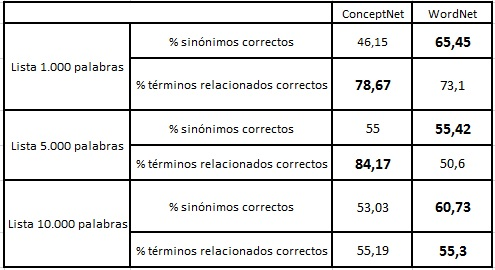
\includegraphics[width=1.0\textwidth]{Imagenes/Bitmap/Capitulo4/tabla_cualitativa}
	\caption{Tabla de resultados de la prueba cualitativa}
	\label{fig:tabla_cualitativa}
\end{figure}

Después del análisis cuantitativo, como se ha descrito en el apartado \ref{cap:subsec:disenioeval} se ha realizado el análisis cualitativo, que consiste en analizar una a una de manera manual, si las palabras obtenidas por ConceptNet y WordNet son correctas(entendiendo como correctas que tengan relación directa con la palabra buscada inicialmente).Como se puede observar, en la Tabla \ref{fig:tabla_cualitativa} los resultados son muy parejos para ambas redes semánticas. En el caso de la comparación con la lista de las 1.000 palabras fáciles, los sinónimos encontrados por WordNet son mejores que los de ConceptNet (65,45\% de sinónimos correctos frente a 46,15\%) sin embargo los términos relacionados son mejores en ConceptNet que en WordNet (78,67\% frente a 73,1\%). Después se hizo la comparación con la lista de 5.000 palabras fáciles, en la que ocurre lo mismo que con la lista anterior, hay más sinónimos correctos en WordNet (55,42\%) que en ConceptNet (55\%) y mejores términos relacionados en ConceptNet (84,17\%) que en WordNet (50,6\%). Por último en las comparaciones realizadas con las 10.000 palabras fáciles los resultados en ambos casos, fueron mejores en WordNet (60,73\% en el caso de los sinónimos y 55,3\% en los términos relacionados) que en ConceptNet (53,03\% y 53,19\% respectivamente).


%-------------------------------------------------------------------
\subsubsection{Conclusiones}
%-------------------------------------------------------------------
\label{sssec:conclusionPruebas}

Valorando los datos obtenidos en ambas pruebas se puede concluir lo siguiente: de la prueba cuantitativa se puede deducir que la red semántica más útil es WordNet ya que en 8 de los 10 parámetros valorados es mejor que ConceptNet. Ya que, aunque el porcentaje de palabras que dejan sin ningún resultado es muy parejo, el número de palabras que deja ConceptNet sin términos relacionados es mucho mayor que el de WordNet(68,75\% frente a 24,72\%, 47,15\% frente a 16,19\% y 43,75 frente a 15,05\%), ocurriendo lo mismo en el caso de los sinónimos(88,06\% frente a 26,5\%, 77,84\% frente a 15,34\% y 76,7\% frente a 9,2\%). En algunos de ellos ganando por una diferencia de más de 60 puntos, por ejemplo, en el porcentaje de palabras sin sinónimos utilizando la lista de las 10.000 palabras fáciles. Además, el número de palabras generadas por WordNet es casi 7 veces mayor que por ConceptNet (14.172 frente a 2.652) lo que supone un factor clave a la hora de elegir que red semántica utilizar finalmente ya que con una se pueden generar muchas más metáforas y símiles que con la otra.

Por otro lado, en la prueba cualitativa realizada, los resultados obtenidos son muy parecidos entre ambas redes semánticas, aunque una vez más, con la que se han obtenido mejores resultados ha sido WordNet ya que ha ganado 4 de los 6 parámetros medidos. Especialmente, en el caso de la lista de las 10.000 palabras, en donde gana ambas mediciones (53,03\% en el caso de los sinónimos correctos con ConceptNet frente a 60,73\% con WordNet y 55,19\% de términos relacionados correctos frente a 55,3\% con ConceptNet y WordNet respectivamente).

Por estos motivos, la red semántica que se ha decidido utilizar finalmente para la aplicación final ha sido WordNet.



 


%-------------------------------------------------------------------
\subsubsection{Servicio Web  para la obtención de  Sinónimos Fáciles}
%-------------------------------------------------------------------
\label{cap:subsec:sw_sinonimosfaciles}

Servicio web que recibe como entrada una palabra y un nivel de búsqueda, y devuelve todos los sinónimos en formato JSON. 

La petición a este servicio sería GET y tendría la siguiente forma:

https://holstein.fdi.ucm.es/tfg-analogias/easysynonym/json/word=\textit{palabra}\&level=\textit{nivel}

Donde \textit{palabra} es el concepto a buscar y \textit{nivel} es el grado de búsqueda, el cual puede tomar los siguientes valores:
\begin{itemize}
	\item Nivel 1 (Nivel sencillo): Se filtran los sinónimos que están entre las 1.000 palabras más usadas de la RAE.
	\item Nivel 2 (Nivel medio): Se filtran los sinónimos que están entre las 5.000 palabras más usadas de la RAE.
	\item Nivel 3 (Nivel avanzado): Se filtran los sinónimos que están entre las 10.000 palabras más usadas de la RAE.
\end{itemize}
 
Una vez introducida la palabra y el nivel, se realiza una consulta a la base de datos a través de una \textit{queryset} para obtener todos los \textit{offsets} cuya palabra sea igual a la introducida.
Si se obtienen resultados, se vuelve a buscar en la base de datos para obtener las palabras de cada \textit{offset}. Por cada palabra obtenida  se comprueba que es distinta del concepto introducido y en función del nivel de búsqueda introducido, se realizará la búsqueda en una de las tres tablas que contienen las palabras fáciles de la RAE y comprobará si alguna de estas palabras se encuentra en dicha tabla.


Si la palabra se encuentra en las palabras más usadas de la RAE, se añade a su correspondiente campo del JSON, y si no se obtiene ningún resultado se devolverá el JSON solamente con un campo que guarda la palabra que se ha introducido.

Por ejemplo, si se realizará una búsqueda para la palabra ``inmueble'' con un nivel de búsqueda 2, la petición GET sería de la siguiente manera:

https://holstein.fdi.ucm.es/tfg-analogias/easysynonym/json/word=inmueble\&level=2

Y en la Figura \ref{fig:peticionGetEasySynonym} se puede ver el resultado obtenido en formato JSON. En primer lugar aparece la palabra buscada, en este caso inmueble y a continuación un objeto que incluye tanto el \textit{offset} como la lista de sinónimos fáciles .

\begin{figure}[!h]
	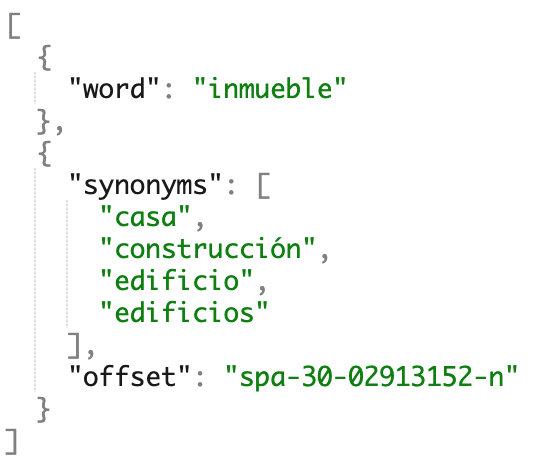
\includegraphics[width=.6\textwidth]{Imagenes/Bitmap/Capitulo5/peticionGetEasySynonym.png}
	\caption{JSON devuelto al buscar los sinónimos fáciles de inmueble en el servicio web para la obtención de sinónimos fáciles}
	\label{fig:peticionGetEasySynonym}
\end{figure}

\figura{Bitmap/Capitulo5/peticionGetEasySynonym}{width=.5\textwidth}{fig:peticionGetEasySynonym}{JSON devuelto al buscar los sinónimos fáciles de inmueble}



%-------------------------------------------------------------------
\subsubsection{Servicio Web  para la obtención de hipónimos fáciles}
%-------------------------------------------------------------------
\label{cap:subsec:sw_hiponimosfaciles}
La implementación de dicho servicio web se basa en que introduciendo una palabra y un nivel de búsqueda, este devuelve todos los hipónimos fáciles correspondientes en formato JSON. Para ello se realiza la siguiente petición GET:

http://127.0.0.1:8000/easyHyponym/json/word=\textit{palabra}\&level=\textit{nivel}

Donde \textit{palabra} es el concepto a buscar y \textit{nivel} es el grado de búsqueda, igual que en el caso explicado anteriormente para buscar sinónimos fáciles.

Una vez introducida la palabra y el nivel, se realiza una consulta a la base de datos de MCR 3.0 a través de una \textit{queryset} para obtener todos los \textit{offsets} cuya palabra sea igual que la introducida.
Por cada \textit{offset} volveremos a buscar en la tabla \textit{Relation} de la base de datos de MCR 3.0 para obtener los offsets que se encuentran en la columna \textit{targetSynset}. Después, con cada \textit{offset} obtenido de esta \textit{queryset}, se realizará la búsqueda en la tabla \textit{Variant} para obtener las palabras cuyo identificador sea igual que el offset de \textit{targetSynset}.
Mediante un cursor se realizará una búsqueda en una de las tres tablas de la RAE (en función del nivel introducido) y buscará si alguna de estas palabras se encuentra en dicha tabla.
Si el resultado es positivo se añadirá al JSON.

Por ejemplo, si se realizará una búsqueda para la palabra inmueble con un nivel de búsqueda 2, la petición GET sería de la siguiente manera:

http://127.0.0.1:8000/easyHyponym/json/word=inmueble\&level=2

Y en la Figura \ref{fig:peticionGetEasyHyponym} se puede ver el resultado obtenido en formato JSON. En primer lugar aparece la palabra buscada, en este caso inmueble y a continuación un objeto que incluye el \textit{offset} de hipónimo fácil , la lista de hipónimos fáciles así como el \textit{offsetFather}, este identificador corresponde al \textit{offset} de uno de los \textit{synsets} de inmueble. De esta forma, si una palabra buscada dispone de varios \textit{synsets}, se podrá mostrar sus correspondientes sinónimos e hipónimos.


\figura{Bitmap/Capitulo5/peticionGetEasyHyponym}{width=1.0\textwidth}{fig:peticionGetEasyHyponym}{JSON devuelto al buscar los hipónimos fáciles de inmueble}
%-------------------------------------------------------------------
\subsubsection{Servicio Web  para la obtención de hiperónimos fáciles}
%-------------------------------------------------------------------
\label{cap:subsec:sw_hiperonimosfaciles}
La implementación de dicho servicio web se basa en que introduciendo una palabra y un nivel de búsqueda, este devuelve todos los hiperónimos fáciles correspondientes en formato JSON. Para ello se realiza la siguiente petición GET:

http://127.0.0.1:8000/easyHyperonym/json/word=\textit{palabra}\&level=\textit{nivel}

Donde \textit{palabra} es el concepto a buscar y \textit{nivel} es el grado de búsqueda, igual que en los casos explicados anteriormente para buscar sinónimos e hipónimos fáciles.

Una vez introducida la palabra y el nivel, se realiza una consulta a la base de datos de MCR 3.0 a través de una \textit{queryset} para obtener todos los \textit{offsets} cuya palabra sea igual que la introducida.
Por cada \textit{offset} volveremos a buscar en la tabla \textit{Relation} de la base de datos de MCR 3.0 para obtener los offsets que se encuentran esta vez y con diferencia de la búsqueda de hipónimos fáciles, en la columna \textit{sourceSynset}. Después, con cada \textit{offset} obtenido de esta \textit{queryset}, se realizará la búsqueda en la tabla \textit{Variant} para obtener las palabras cuyo identificador sea igual que el offset de \textit{sourcetSynset}.
Mediante un cursor se realizará una búsqueda en una de las tres tablas de la RAE (en función del nivel introducido) y buscará si alguna de estas palabras se encuentra en dicha tabla.
Si el resultado es positivo se añadirá al JSON.

Por ejemplo, si se realizará una búsqueda para la palabra inmueble con un nivel de búsqueda 2, la petición GET sería de la siguiente manera:

http://127.0.0.1:8000/easyHyperonym/json/word=inmueble\&level=2

En la Figura \ref{fig:peticionGetEasyHyperonym} se puede ver el resultado obtenido en formato JSON. En primer lugar aparece la palabra buscada, en este caso inmueble y a continuación un objeto que incluye el \textit{offset} de hiperónimo fácil, la lista de hiperónimos fáciles así como el \textit{offsetFather}, ya explicado en el apartado anterior.


\figura{Bitmap/Capitulo5/peticionGetEasyHyperonym}{width=1.0\textwidth}{fig:peticionGetEasyHyperonym}{JSON devuelto al buscar los hiperónimos fáciles de inmueble}
%-------------------------------------------------------------------
\subsubsection{Servicio Web  para la obtención de metáforas}
%-------------------------------------------------------------------
\label{cap:subsec:sw_metaforas}
Este servicio web dado un offset y una profundidad obtiene las metáforas de un concepto, es decir, se obtienen tanto los sinónimos como los hiperónimos fáciles formando la metáfora y este servicio devuelve dichos resultados en formato JSON.
Para ello se realiza la siguiente petición GET:

http://127.0.0.1:8000/metaphor/json/word=\textit{palabra}\&level=\textit{nivel}

Donde \textit{palabra} es el concepto a buscar y \textit{nivel} es el grado de búsqueda, igual que en los casos explicados anteriormente para buscar sinónimos, hipónimos e hiperónimos fáciles.

La implementación de dicho servicio es idéntico al ya explicado en el servicio web para obtener sinónimos fáciles e hiperónimos fáciles, con la única diferencia que para poder formar la metáfora se llama a otro servicio implementado, el cual utiliza SpaCy para definir si el concepto es masculino o femenino y si está en singular o plural.

Por ejemplo, si se realizará una búsqueda para la palabra inmueble con un nivel de búsqueda 2, la petición GET sería de la siguiente manera:

http://127.0.0.1:8000/metaphor/json/word=inmueble\&level=2

En la Figura \ref{fig:peticionMetaphor} se puede ver el resultado obtenido en formato JSON. En primer lugar aparece la palabra buscada, en este caso inmueble y a continuación un objeto que incluye el \textit{offset} del sinónimo o hiperónimo fácil, el \textit{offsetFather}  ya explicado en apartados anteriores y la lista de metáforas (es una casa, es una construcción, son unos edificios, es un edificio). 


\figura{Bitmap/Capitulo5/peticionMetaphor}{width=1.0\textwidth}{fig:peticionMetaphor}{JSON devuelto al buscar las metáforas de la palabra inmueble}
%-------------------------------------------------------------------
\subsubsection{Servicio Web  para la obtención de símiles}
%-------------------------------------------------------------------
\label{cap:subsec:sw_simil}
Este servicio web dado un offset y una profundidad obtiene los símiles de un concepto, es decir, se obtienen los hipónimos fáciles formando así el símil y devolviendo los resultados en formato JSON.
Para ello se realiza la siguiente petición GET:

http://127.0.0.1:8000/simil/json/word=\textit{palabra}\&level=\textit{nivel}

Donde \textit{palabra} es el concepto a buscar y \textit{nivel} es el grado de búsqueda, igual que en los casos explicados anteriormente.
Para la implementación de dicho servicio, se utiliza exactamente el mismo código explicado en el apartado de obtención de hipónimos fáciles pero incluyendo la llamada al servicio de SpaCy para volver a definir si el concepto es masculino o femenino y si es singular o plural.

Por ejemplo, si se realizará una búsqueda para la palabra inmueble con un nivel de búsqueda 2, la petición GET sería de la siguiente manera:

http://127.0.0.1:8000/simil/json/word=inmueble\&level=2

En la Figura \ref{fig:peticionSimil} se puede ver el resultado obtenido en formato JSON. En primer lugar aparece la palabra buscada, en este caso inmueble y a continuación un objeto que incluye el \textit{offset} del hipónimo fácil, el \textit{offsetFather}  ya explicado en apartados anteriores y la lista de símiles (es como una biblioteca es como un colegio, es como un restaurante).


\figura{Bitmap/Capitulo5/peticionSimil}{width=1.0\textwidth}{fig:peticionSimil}{JSON devuelto al buscar los símiles de la palabra inmueble}


%-------------------------------------------------------------------
\subsection{Frontend  de Aprende Fácil}
%-------------------------------------------------------------------
Igual que la parte interna de una aplicación es de suma importancia, la parte visual y como el usuario interactúa con ella es una parte a tener en cuenta siempre. Para este trabajo, como se ha comentado en la sección \ref{cap:sec:disenioInterfaz}  se necesita aún más tener en cuenta cuales son los usuarios finales y sus necesidades, por lo que la interfaz debe adecuarse a ellos.
Lo primero que debemos decir respecto a la implementación, es que para la creación de los elementos visuales de la interfaz, así como para la colocación de los distintos elementos se ha uso de HTML, CSS y Bootstrap4 y para el funcionamiento de los distintos elementos así como para obtener los resultados que proporcionan los servicios web se ha hecho uso de JavaScript y jQuery.

En la Figura \ref{fig:paginaInicial} se puede ver la interfaz de la aplicación final sin haber buscado aún ningún concepto. Se han numerado los elementos principales y a continuación se explicarán detalladamente:

\begin{figure}[!h]
	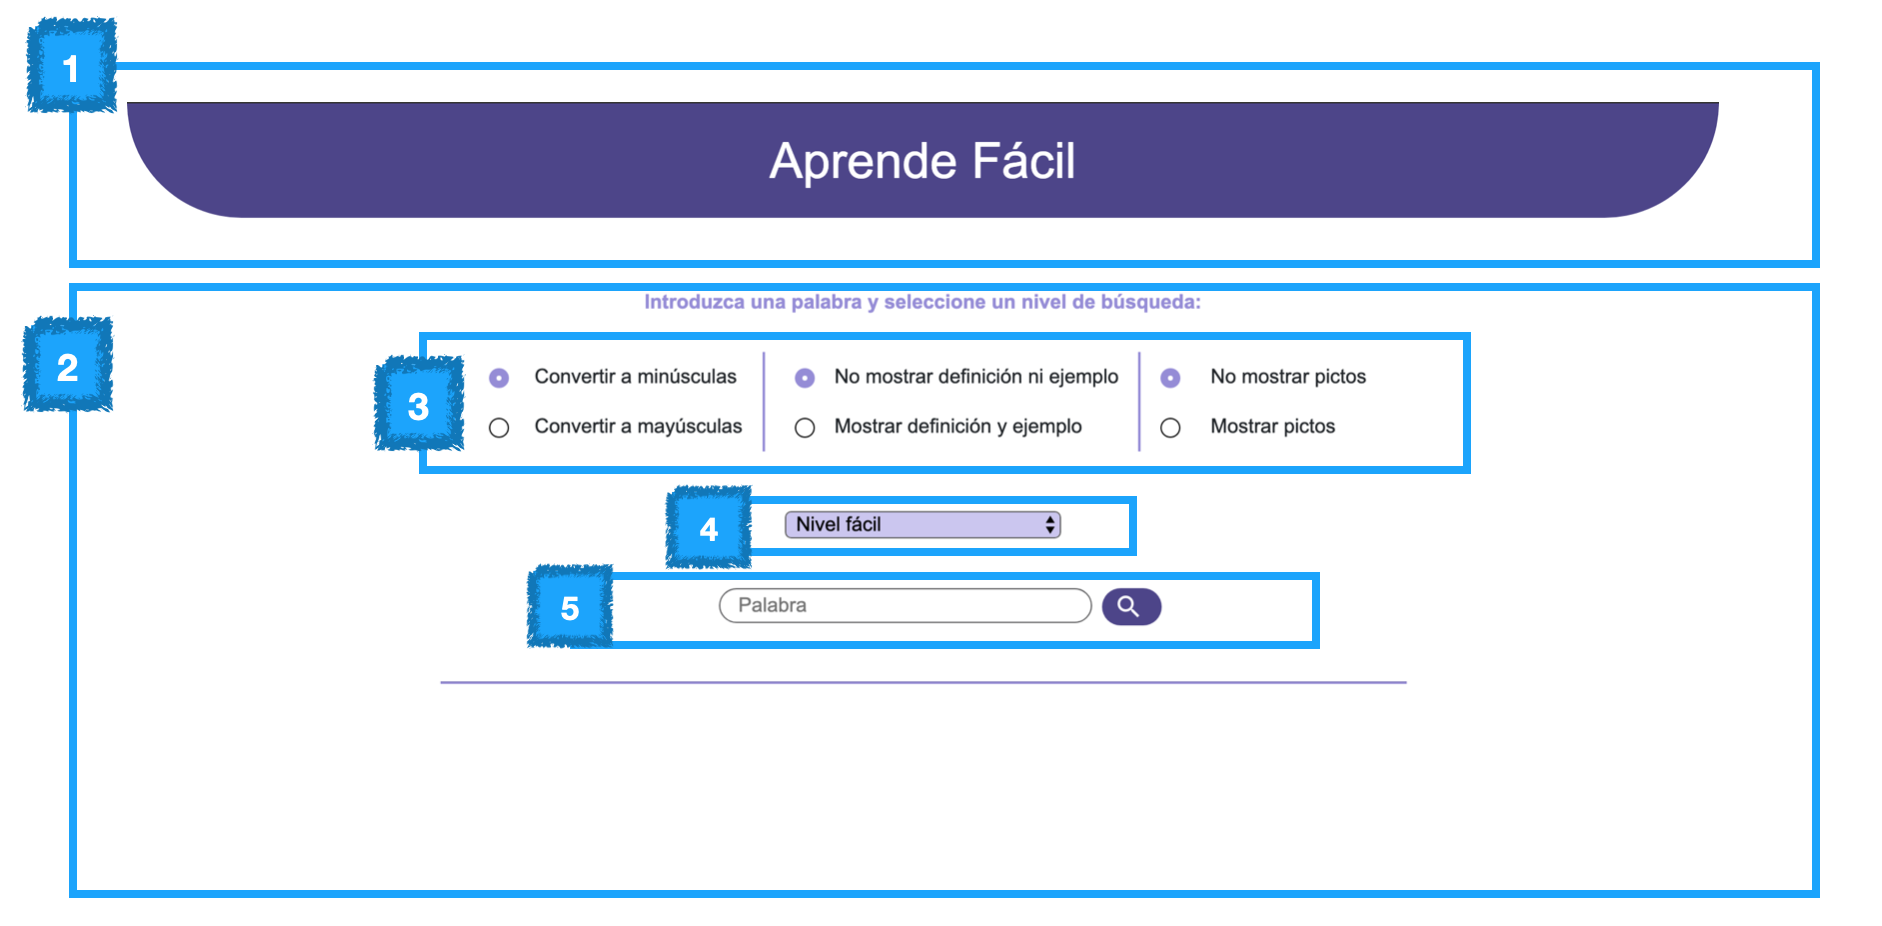
\includegraphics[width=1.2\textwidth]{Imagenes/Bitmap/Capitulo4/Frontend/paginaInicial.png}
	\caption{Interfaz de Aprende Fácil  sin realizar ninguna búsqueda}
	\label{fig:paginaInicial}
\end{figure}


\begin{itemize}
	\item Elemento número 1 - Barra de navegación: Para la barra de navegación se ha utilizado la etiqueta <nav> propia de Bootstrap4 y para que los laterales queden redondeados se añadió al estilo la propiedad ``radius'' tanto en el borde inferior izquierdo como en el borde inferior derecho.
	\item Elemento número 2 - Contenedor: El contenedor engloba toda la página exceptuando la barra de navegación, para ello se añade la clase ``container'', también propia de Bootstrap4 y dentro de este es donde se implementan el resto de elementos que forman la interfaz.
	\item Elemento número 3 - Selectores tipo ``radio'': Para la implementación de este elemento, se creó un <div> para cada par de opciones de configuración (Por ejemplo, Convertir a minúsculas y Convertir a mayúsculas) añadiéndole una clase que contiene un estilo CSS para que los elementos se ordenen por columna, es decir, uno debajo de otro. Además se le añadió un ``checkbox'' de tipo radio para poder seleccionar una opción u otra pero no ambas a la vez.
	\item Elemento número 4 - Desplegable con opciones: Este desplegable se encuentra dentro de otra etiqueta <div> con una etiqueta <select> propia de Bootstrap4 y que permite añadir un listado con distintas opciones. En este caso sirve para que el usuario pueda decidir con que nivel de búsqueda quiere realizar la consulta. A parte, se le añadió un estilo para que el elemento quede centrado en la página.
	\item Elemento número 5 - Entrada de texto y botón enviar: La barra para introducir la palabra es un <input> de tipo texto, al cual se le añadió una propiedad CSS ``radius'' para redondear los bordes y un ``placeholder'' con el texto ``Palabra'' para que el usuario sepa que debe introducir. Y por otro lado, se encuentra el botón con un icono de una lupa pero que al pasar el ratón por encima tiene un efecto y el botón se alarga, añadiendo a este icono la palabra Buscar.
	Tanto el input como el botón están dentro de un <div> que contiene un estilo para centrar ambos elementos.
\end{itemize}

Se ha intentado separar mediante una barra el panel de arriba donde se encuentra la configuración de la aplicación y el panel abajo donde se muestran los resultados. 
Ahora que ya se ha explicado la implementación de los elementos estáticos de la interfaz, explicaremos como se crean de manera dinámica el resto de elementos.
En la Figura \ref{fig:paginaResultado} se encuentra la aplicación con los resultados para la palabra ``Familia''. En esta Figura se han vuelto a enumerar los elementos para poder comprender mejor como funciona la aplicación. 
Para este ejemplo se ha seleccionado las opciones ``Mostrar pictos'' y ``Mostrar definición y ejemplo'', y cuando se introduce una palabra y se da al botón de Buscar, se realiza una petición AJAX la cuál se conecta con el Backend y obtiene un JSON formado por cuatro objetos: todos los \textit{offsets} de la palabra buscada, las metáforas, los símiles y las definiciones y ejemplos. Por cada \textit{offset} se comprueba mediante JavaScript que \textit{offset} de metáfora coincide y que \textit{offset} de símil coincide y así poder mostrarlos en una misma ficha.
A continuación, se explicarán como se construye cada elemento:


\begin{figure}[!h]
	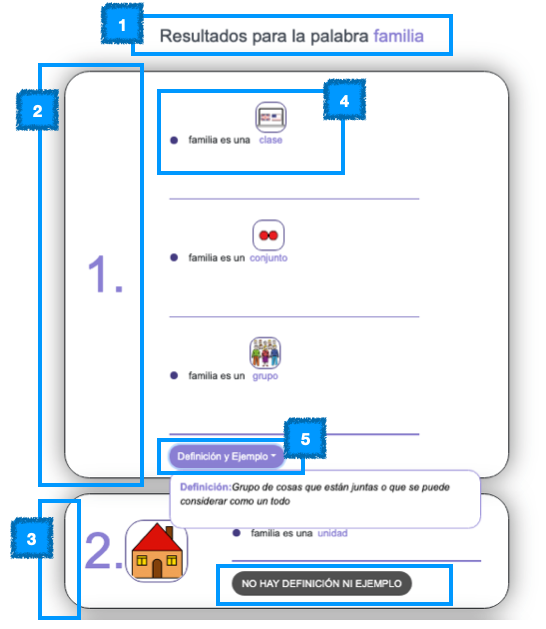
\includegraphics[width=.9\textwidth]{Imagenes/Bitmap/Capitulo4/Frontend/paginaResultado.png}
	\caption{Interfaz de Aprende Fácil mostrando resultados }
	\label{fig:paginaResultado}
\end{figure}


\begin{itemize}
	\item Elemento número 1 - Texto informativo: Da información constante de la palabra que se ha buscado. En caso de que la palabra introducida sea inventada aparecerá ``No hay resultados para la palabra X''. Este texto informativo se añade a la interfaz mediante jQuery una vez que se ha realizado la petición AJAX y se puede saber si tiene o no resultados.
	
	\item Elemento número 2 y 3 - Ficha: Como se ha explicado anteriormente, hay que mostrar los resultados según su significado, por lo que la relación entre el significado de la palabra buscada, y el significado de la palabra mostrada es el \textit{offset}. Con JavaScript se recorre \textit{offset} a \textit{offset}, y por cada uno de ellos se comprueba que resultados tienen el mismo identificador. Esta ficha se crea dinamicamente según el número de resultados que se obtengan y es un <div> con una clase donde se añade un estilo para redondear los bordes, y la propiedad ``box-shadow'' para el sombreado, dando así sensación de que la ficha está superpuesta a la página. A parte, se debe saber si el resultado principal dispone de pictograma o no, por lo que se mediante la siguiente url ``https://holstein.fdi.ucm.es/tfg-analogias/imagen/\textit{offset}'' donde \textit{offset} es el identificador, se realiza una petición GET al servicio web correspondiente.
	
	\item Elemento número 4 - Resultado en formato lista: Como se puede observar los resultados se muestran en formato lista, primero aparecen las metáforas y después los símiles. Para poder obtener la frase completa, se recoge la metáfora (en este caso ``familia es una grupo'') se realiza un \textit{split} para poder quedarnos con la última palabra y se vuelve hacer una petición GET al servicio web con la siguiente url ``https://holstein.fdi.ucm.es/tfg-analogias/imagenByPalabra/\textit{palabra}'' donde palabra, siguiendo con el ejemplo anterior sería ``grupo'' y así se obtiene el pictograma correspondiente.
	
	\item Elemento número 5 - Botón definición y ejemplo: Se muestra la definición y ejemplo cuyo \textit{offset} concida con el \textit{offset} de la ficha principal. En caso de que no tenga se mostrará ``NO HAY DEFINICIÓN NI EJEMPLO''. Este botón siempre aparecerá después de mostrar todas las metáforas y símiles.
 
\end{itemize}


Cabe destacar que una vez mostrados los resultados, tenemos la posibilidad de ocultar o mostrar los pictogramas así como la definición y el ejemplo sin tener que volver a realizar la búsqueda. Esto se consigue teniendo un manejador de eventos, el cual una vez que se pincha sobre los diferentes ``checkbox'' se añaden o eliminar las clases necesarias para que la interfaz se vea siempre correctamente. Por ejemplo, si en la Figura se pulsara sobre ``Ocultar pictos'', estos desaparecían y la palabra se quedaría perfectamente alineada con el texto de la metáfora. En el caso de pinchar sobre ``Convertir a mayúsculas'' se le añadiría un estilo CSS a la etiqueta <body>con la propiedad ``text-transform: uppercase''.
Por último, también se puede realizar la búsqueda de algún resultado obtenido pinchando sobre el, haciendo así que se vuelva a realizar una petición AJAX, recogiendo los resultados que se han comentado anteriormente y siguiendo el mismo proceso para mostrar los resultados.

%-------------------------------------------------------------------
\section{Evaluación de Aprende Fácil}
%-------------------------------------------------------------------

El día 17 de Mayo de 2019 a las 10:30h tuvo lugar la evaluación final en el colegio Estudio3 Afanias\footnote{https://afanias.org/que-hacemos/educacion/colegio-estudio-3/} situado en la Comunidad de Madrid. Este colegio era el mismo donde se realizó la evaluación con los expertos explicado en la sección \ref{cap:subsec:evaluacionExpertos}. A esta evaluación acudieron los integrantes del equipo junto con los directores.

La evaluación se realizó con dos grupos: El primer grupo formado por 7 alumnos de la edad de 17 años y 1 profesor, y un segundo grupo formado por 7 alumnos de la edad de 14 años y 1 profesor.
Cabe destacar que el primer grupo estaba formado mayoritariamente por alumnos autónomos e independientes, en contraposición del segundo grupo que tenían un mayor grado de discapacidad.
En un primer momento se realizó un formulario de Google Forms, dividido en dos secciones: Una primera sección guiada enfocada al análisis de los resultados, viendo si estos eran útiles y correctos.  Y otra sección dedicada a la usabilidad de la aplicación.
Dicho formulario  puede encontrarse en nuestro repositorio de GitHub, y en el Ápendice ..X..

La idea principal era que cada usuario probará la aplicación y realizara el formulario de forma individual, pero finalmente se decidió que los integrantes del equipo fueran los que realizaran la evaluación in situ mientras los alumnos daban su opinión y se recogían sus respuestas.
La primera sección del formulario se dividía en distintas pruebas según lo que se quería evaluar, a continuación se  
\begin{itemize}
	\item PRUEBA 1 - Búsqueda con nivel fácil: La primera palabra introducida fue ``PUENTE'' con un nivel de búsqueda fácil y con las opciones de pictograma y definición y ejemplo predeterminadas. En la Figura  \ref{fig:puenteFacil} se pueden ver los resultados obtenidos, donde los alumnos comprendían tanto el resultado ``construcción'' como ``estructura'' . Y nos comentaron que les pareció bastante útil puesto que les ayudaba aún más a comprender el significado del concepto buscado.

		\begin{figure}[!h]
		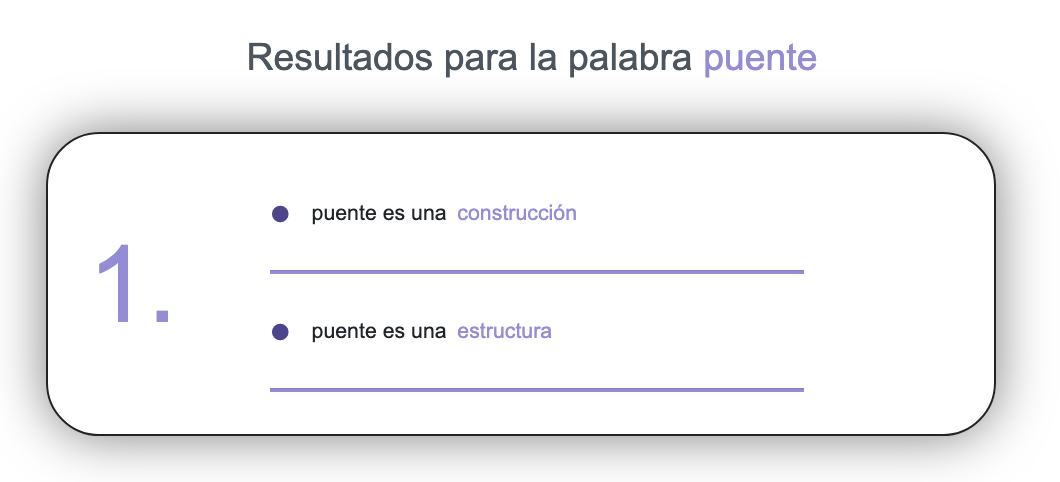
\includegraphics[width=.7\textwidth]{Imagenes/Bitmap/Capitulo4/EvaluacionFinal/1puentefacil.png}
		\centering
		\caption{Resultado obtenido para la palabra ``Puente'' con un nivel de búsqueda fácil}
		\label{fig:puenteFacil}
		\end{figure}
	
	\item PRUEBA 2 - Búsqueda con nivel medio: Se introdujo la misma palabra ``PUENTE'' pero aumentando el nivel de búsqueda a medio. En la Figura \ref{fig:puenteMedio} se pueden ver los resultados obtenidos. En este caso hubo que explicar a los alumnos los dos nuevos resultados. Por un lado, para la palabra ``arco'' no entendían la relación existente de este  con la palabra buscada y por otro lado, para la palabra ``circuito'' relacionaban dicho concepto con un circuito de carreras en vez de un circuito electrónico, siendo este último el significado obtenido por la aplicación.
	
		\begin{figure}[!h]
		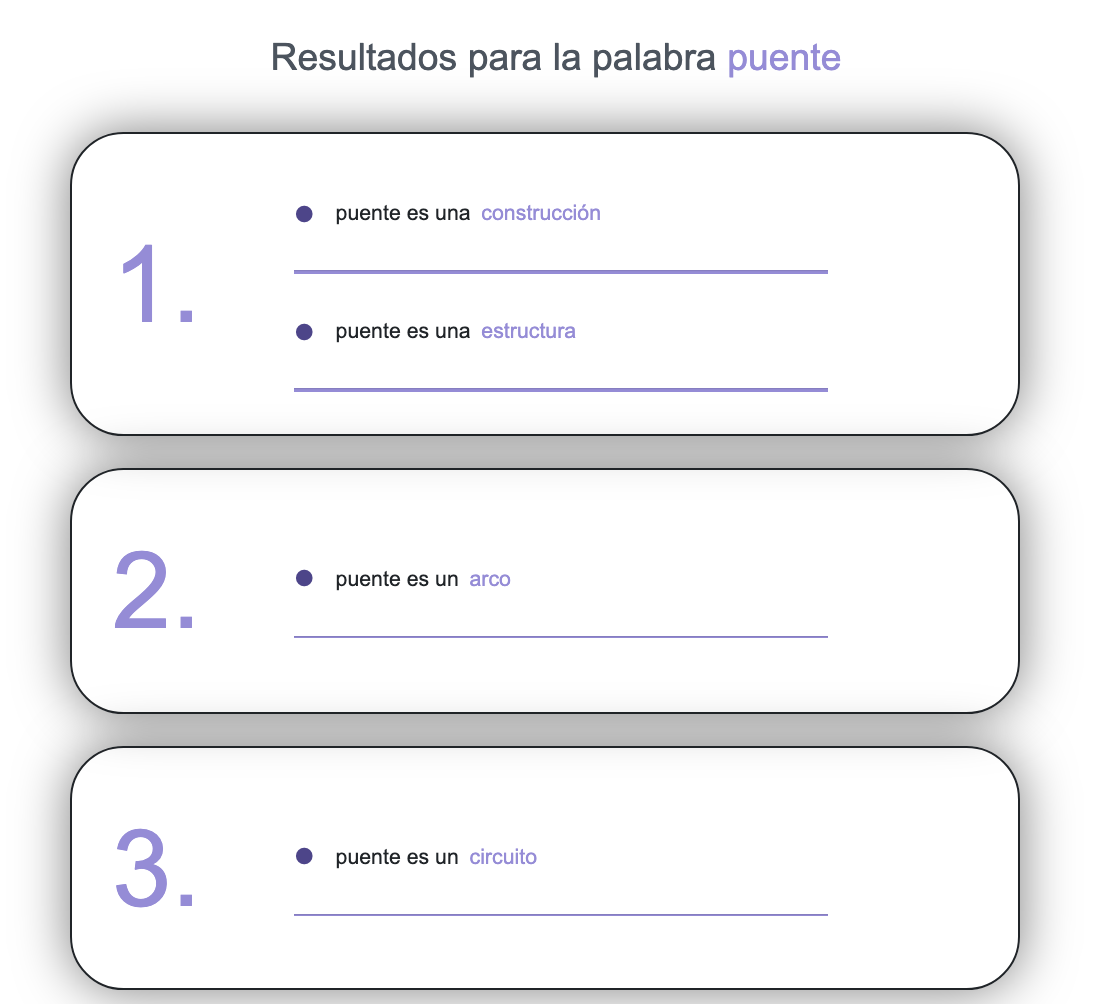
\includegraphics[width=.7\textwidth]{Imagenes/Bitmap/Capitulo4/EvaluacionFinal/2puentemedio.png}
		\centering
		\caption{Resultado obtenido para la palabra ``Puente'' con un nivel de búsqueda medio}
		\label{fig:puenteMedio}
		\end{figure}


	\item PRUEBA 3 - Búsqueda con nivel avanzado: Esta vez, se volvió a introducir la palabra ``PUENTE'' con un nivel de búsqueda avanzado. En la Figura  \ref{fig:puenteAvanzado} se pueden ver los resultados obtenidos donde se puede ver que con este nivel se muestra un resultado más que en el anterior nivel. La palabra ``placa'' puede tener diversos significados según el contexto en el que se utilice, por lo que para los alumnos era complicado entender la relación de ``placa'' con ``puente''. Una vez explicado, los alumnos entendieron perfectamente su significado.
		\begin{figure}[!h]
		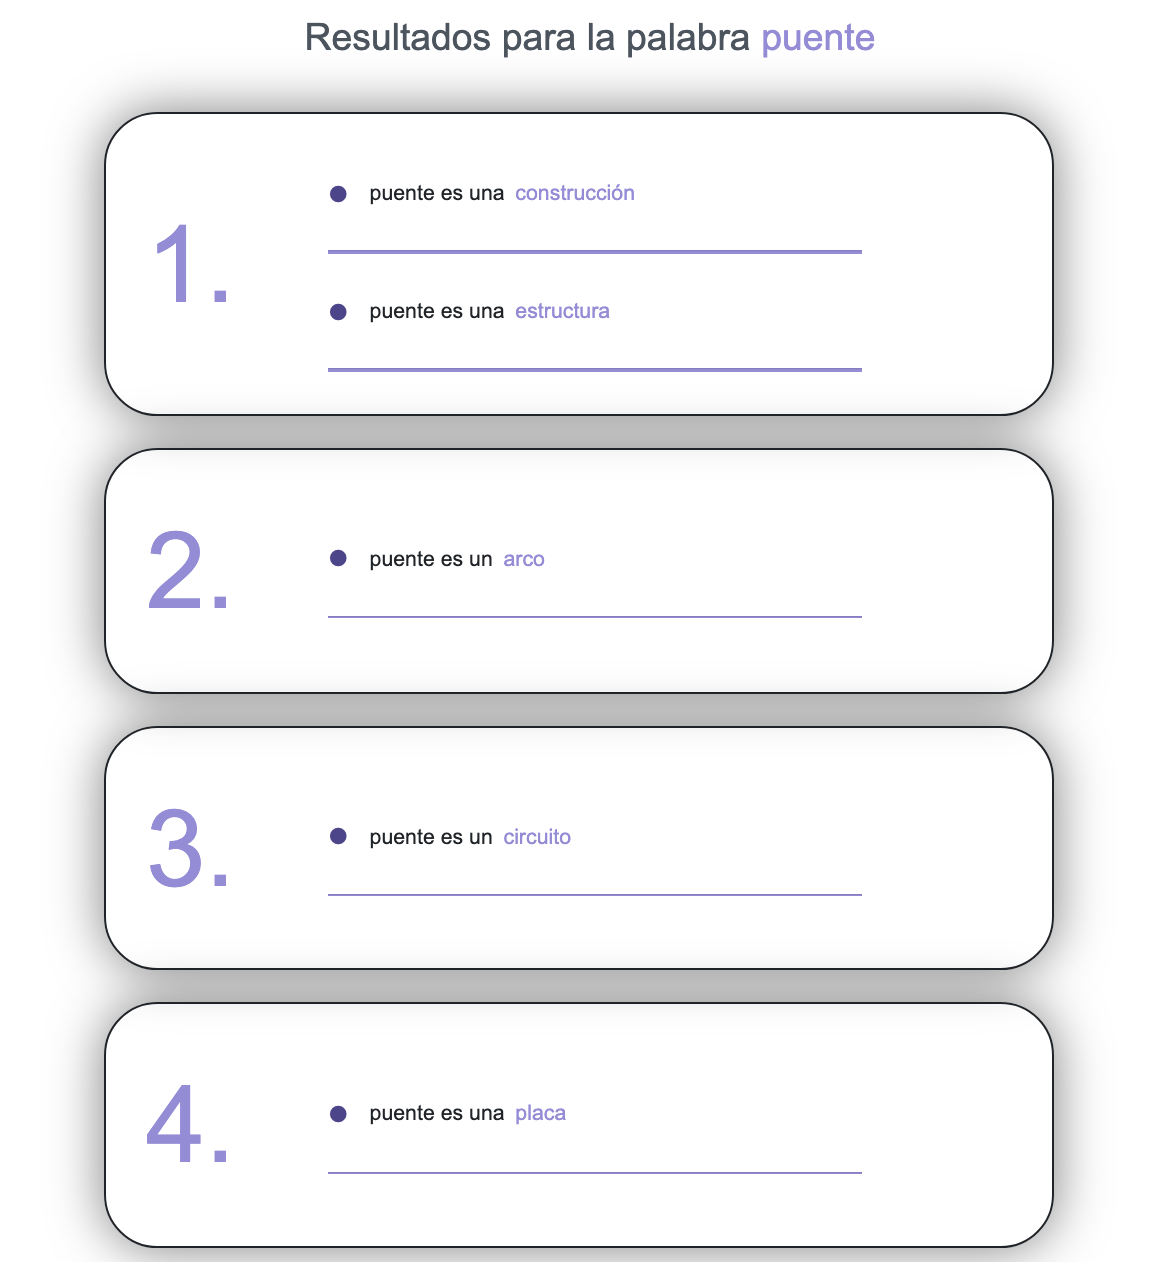
\includegraphics[width=.7\textwidth]{Imagenes/Bitmap/Capitulo4/EvaluacionFinal/3puenteavanzado.png}
		\centering
		\caption{Resultado obtenido para la palabra ``Puente'' con un nivel de búsqueda avanzado}
		\label{fig:puenteAvanzado}
		\end{figure}
	
	\item PRUEBA 4 - Obteniendo un único resultado: La palabra introducida fue ``DICTADOR'' con un nivel de búsqueda avanzado y sin mostrar ni pictogramas ni definición y ejemplo. En la Figura \ref{fig:dictadorAvanzado} se pueden ver los resultados obtenidos, de estos comprendieron el resultado ``lider'' pero no sabían que era ``soberano''. De los demás resultados obtenidos, entendían ``gobernador'' pero no sabían la diferencia que existía entre este y ``gobernante'', lo que les llevo a confusión no dejando claro el significado del concepto.
	
		\begin{figure}[!h]
			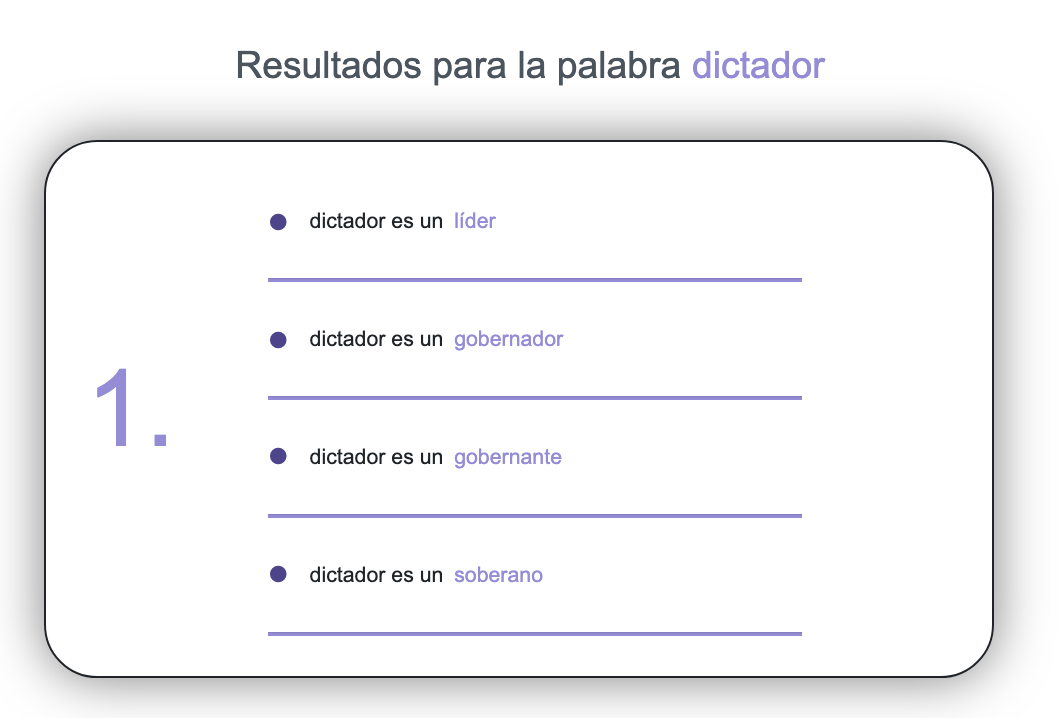
\includegraphics[width=.7\textwidth]{Imagenes/Bitmap/Capitulo4/EvaluacionFinal/4dictadoravanzado.png}
			\centering
			\caption{Resultado obtenido para la palabra ``Dictador'' con un nivel de búsqueda avanzado}
			\label{fig:dictadorAvanzado}
		\end{figure}
	
	\item PRUEBA 5 - Obteniendo varios resultados (I):  Se introdujo la palabra ``DEFENSA'' con un nivel de búsqueda fácil. En la Figura \ref{fig:defensaFacil} se pueden ver los resultados obtenidos donde los alumnos entendían todos. Para profundizar aún más, en esta búsqueda se añadió la opción de mostrar pictogramas, la respuesta de los alumnos fue que los resultados se entienden de una manera más clara y sencilla, ya que les ayuda a entender el significado según el contexto en el que se está utilizando.
		
			\begin{figure}[!h]
			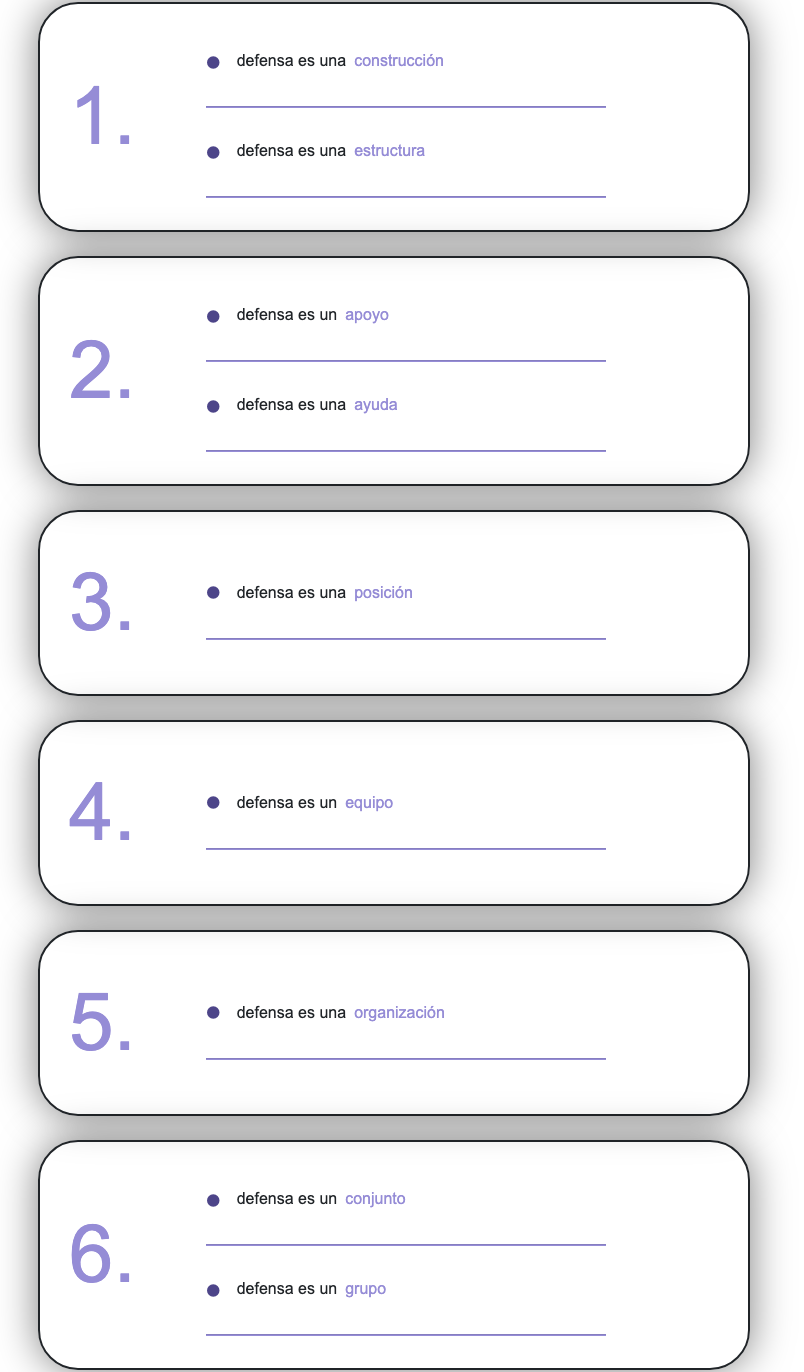
\includegraphics[width=.7\textwidth]{Imagenes/Bitmap/Capitulo4/EvaluacionFinal/5defensafacil.png}
			\centering
			\caption{Resultado obtenido para la palabra ``Defensa'' con un nivel de búsqueda fácil}
			\label{fig:defensaFacil}
		\end{figure}
	
	\item PRUEBA 6 - Obteniendo varios resultados (II):  Se realizó otra prueba para obtener varios resultados. En este caso de introdujo la palabra ``DANZA''  sin pictogramas y con un nivel de búsqueda avanzado. En la Figura \ref{fig:danzaAvanzado} se pueden ver los resultados obtenidos, de los cuales los alumnos entendieron todos sin ningún problema.
	
	\begin{figure}[!h]
		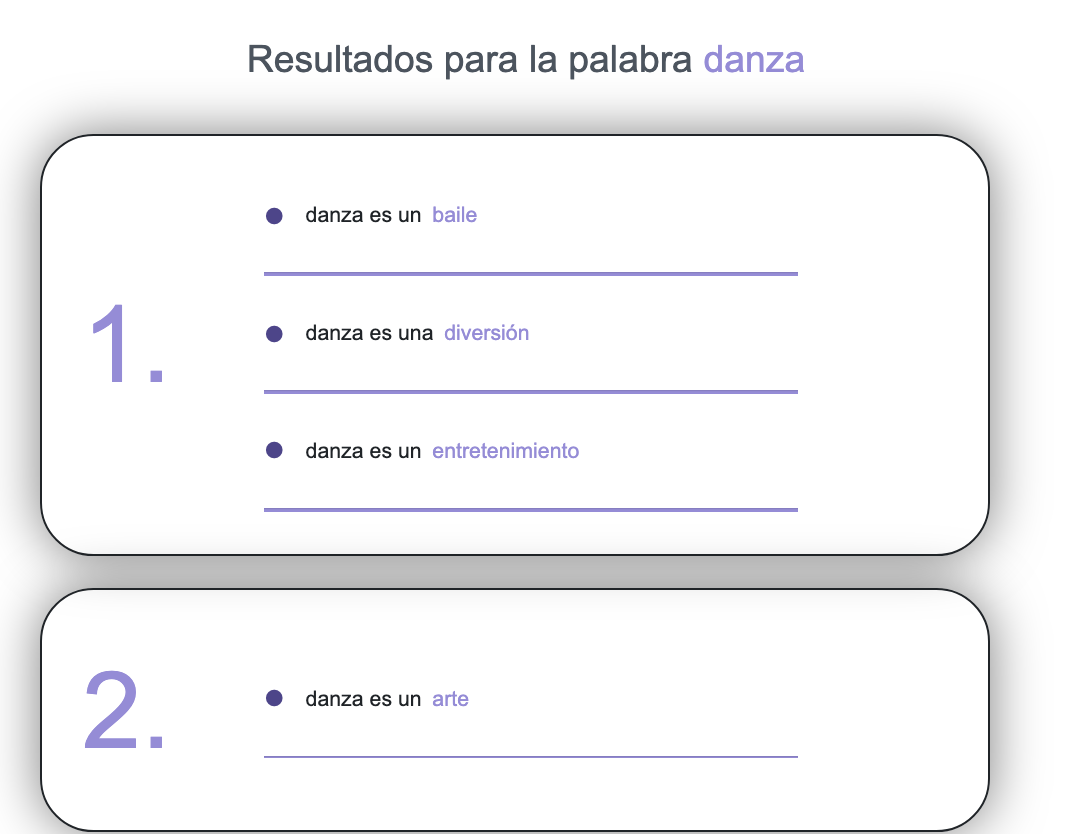
\includegraphics[width=.7\textwidth]{Imagenes/Bitmap/Capitulo4/EvaluacionFinal/6danzaavanzado.png}
		\centering
		\caption{Resultado obtenido para la palabra ``Danza'' con un nivel de búsqueda avanzado}
		\label{fig:danzaAvanzado}
	\end{figure}
	
	\item PRUEBA 7 - Obtención de metáforas:  Se introdujo la palabra ``PORTERO'' con un nivel de búsqueda avanzado y añadiendo la opción de mostrar pictogramas. Se puede ver en la Figura \ref{fig:porteroAvanzado} los resultados obtenidos. Todos fueron correctos excepto para el resultado ``funcionario'' y ``administrador'', que no entendían su significado. Después, se cambio el nivel de búsqueda a medio, para saber si con un nivel inferior donde se obtendrían menos resultados, les era más sencillo entenderlo. De esta forma se obtuvieron dos resultados: ``Portero es un guardia'' y ``Portero es un funcionario'' de los cuales el primero lo entendieron y el segundo solamente si se añade la opción de mostrar pictograma.
	
	\begin{figure}[!h]
		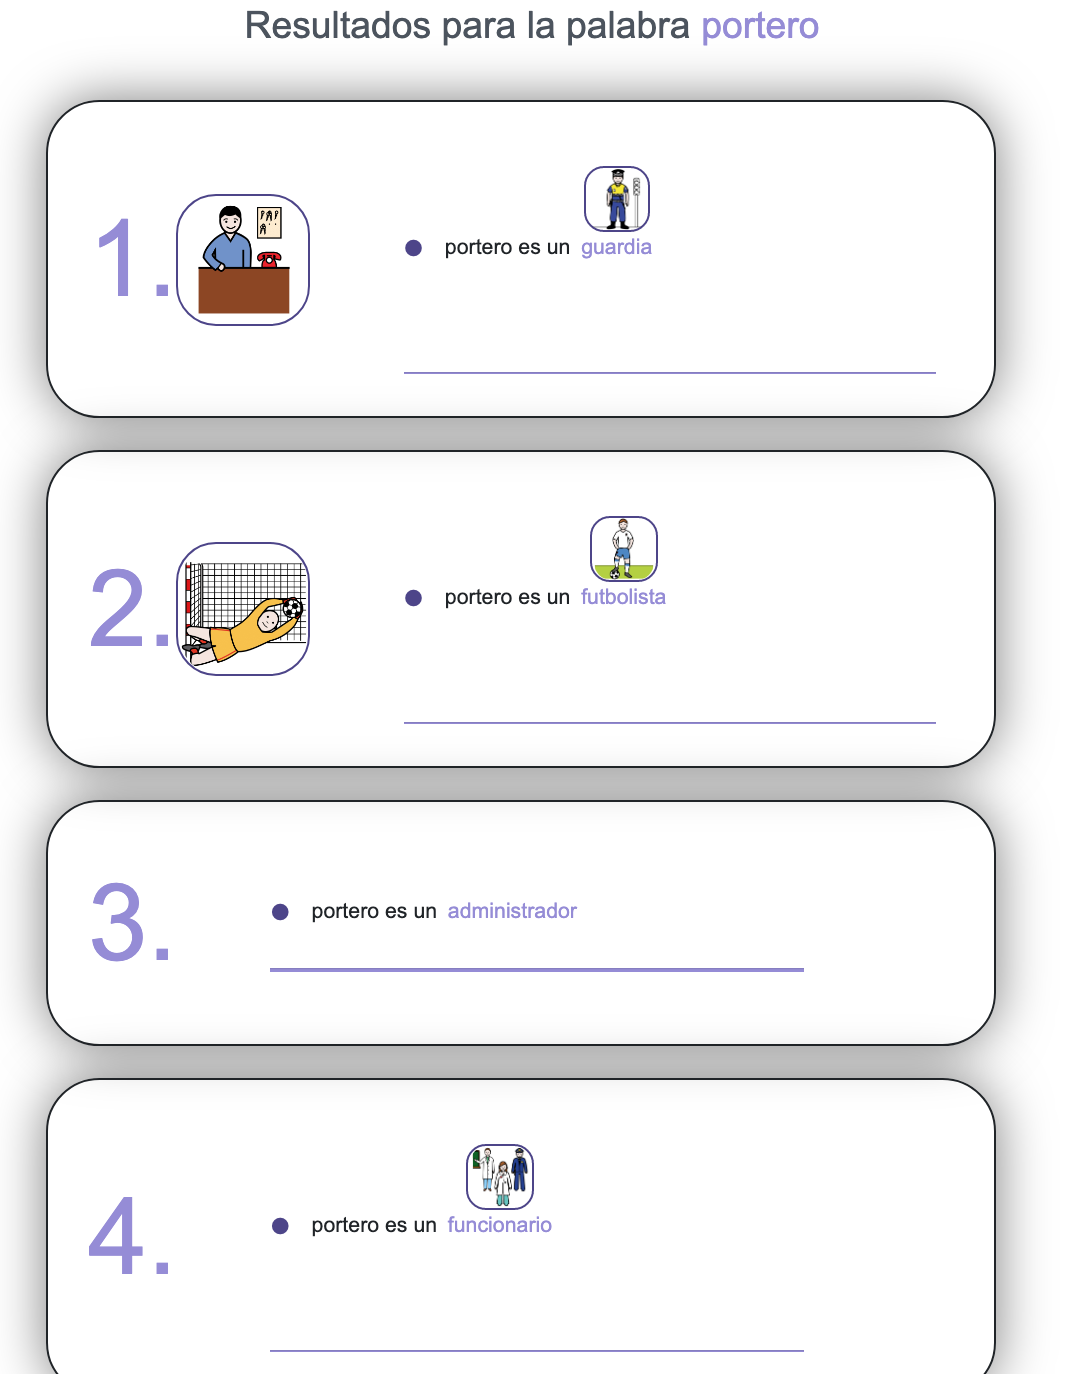
\includegraphics[width=.7\textwidth]{Imagenes/Bitmap/Capitulo4/EvaluacionFinal/7porteroavanzadopictos.png}
		\centering
		\caption{Resultado obtenido para la palabra ``Portero'' con un nivel de búsqueda avanzado y mostrando pictogramas}
		\label{fig:porteroAvanzado}
	\end{figure}

\item PRUEBA 8 - Obtención de símiles:  Se introdujo la palabra ``FUNCIONARIO'' con un nivel de búsqueda fácil. Se puede ver en la Figura \ref{fig:funcionarioFacil} los resultados obtenidos, donde todos fueron comprendidos perfectamente por los alumnos. 

\begin{figure}[!h]
	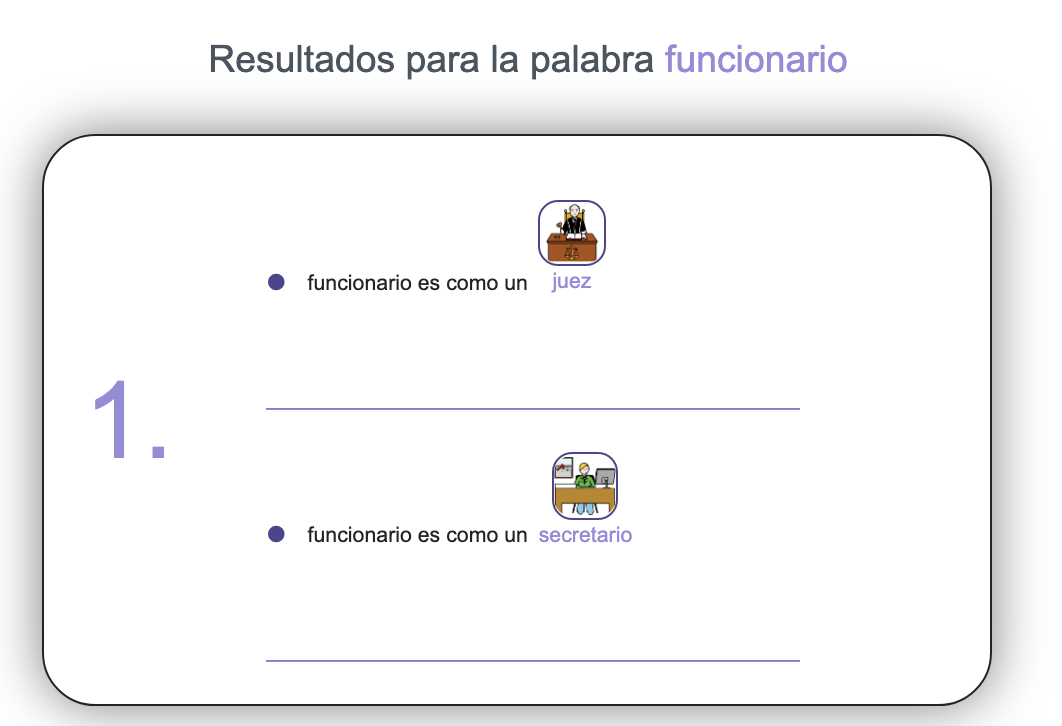
\includegraphics[width=.7\textwidth]{Imagenes/Bitmap/Capitulo4/EvaluacionFinal/8funcionariofacil.png}
	\centering
	\caption{Resultado obtenido para la palabra ``Funcionario'' con un nivel de búsqueda fácil}
	\label{fig:funcionarioFacil}
\end{figure}


\item PRUEBA 9 - Definición y ejemplo:  Se buscó la palabra ``FAMILIA'' con un nivel de búsqueda fácil y añadiendo la opción de mostrar definición y ejemplo. Se puede ver en la Figura \ref{fig:familiaFacilDef} los resultados obtenidos, De estos, en la primera ficha no entienden el resultado ``clase'' pero si les ayuda la definición \textit{(``Grupo de cosas que están juntas o que se puede considerar como un todo'')}. Igual ocurre en la ficha tres pero con el resultado ``línea'' \textit{(``Descendientes de un individuo'')}, donde ellos entienden línea como una recta, pero leyendo la definición comprenden que se refiere a línea sucesoria.

\begin{figure}[!h]
	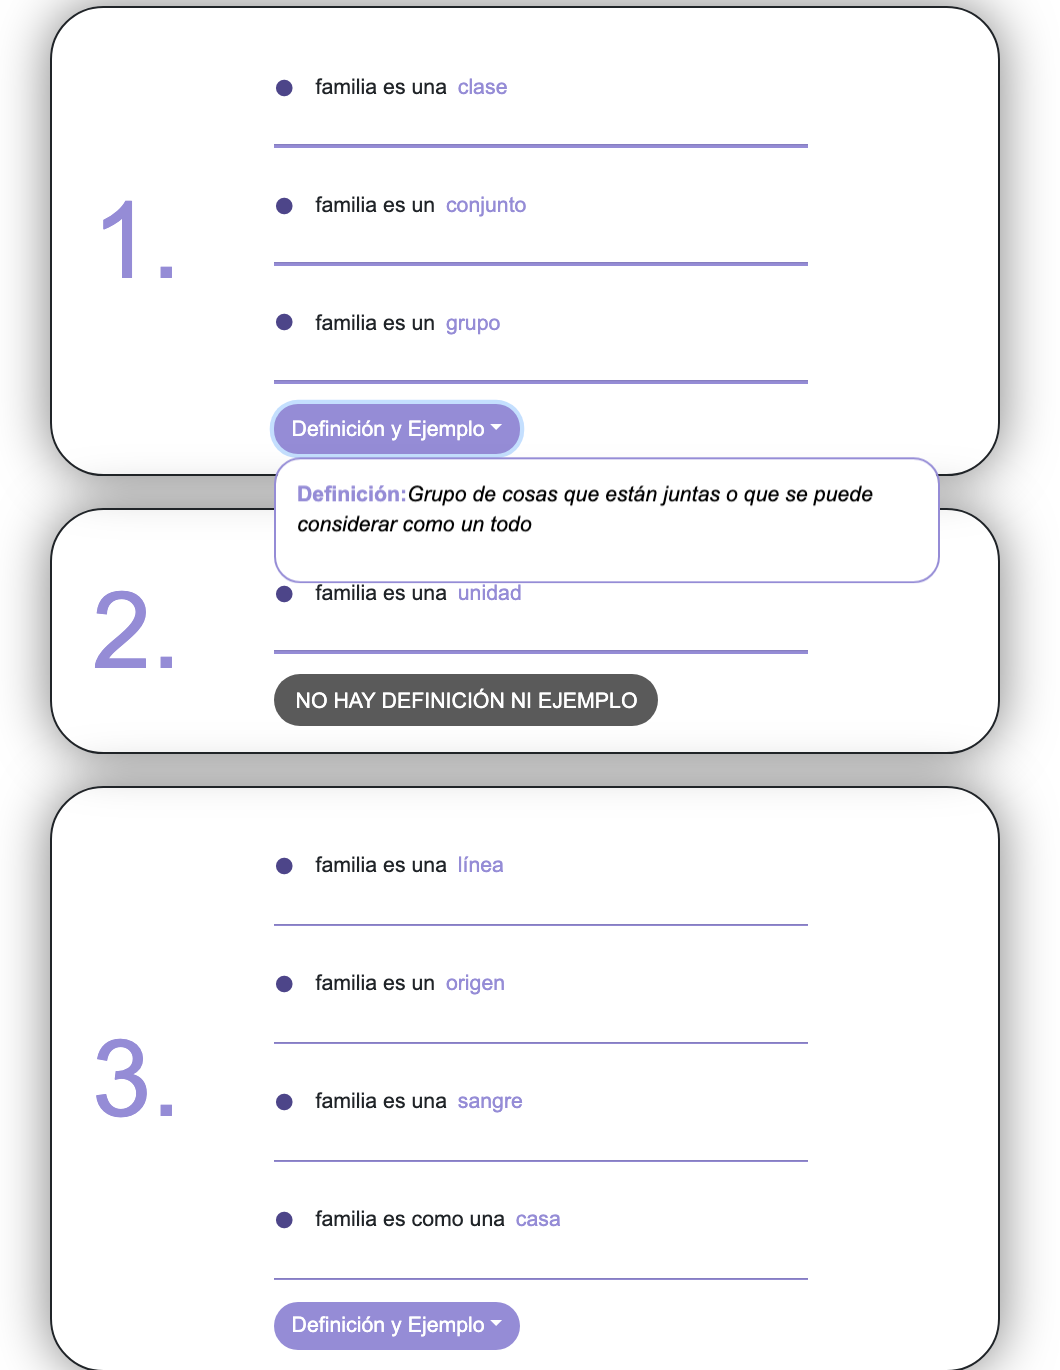
\includegraphics[width=.7\textwidth]{Imagenes/Bitmap/Capitulo4/EvaluacionFinal/9familiafacildef.png}
	\centering
	\caption{Resultado obtenido para la palabra ``Familia'' con un nivel de búsqueda fácil y añadiendo la opción ``Mostrar definición y ejemplo''}
	\label{fig:familiaFacilDef}
\end{figure}
 
\item PRUEBA 10 - Uso de mayúsculas:  Con la misma palabra ``FAMILIA'', se realizó el cambio de minúsculas a mayúsculas como se puede ver en la Figura \ref{fig:familiaMayusculas}, los alumnos nos comentaron que prefieren esta opción puesto que están más familiarizados y es como aprenden a escribir.

\begin{figure}[!h]
	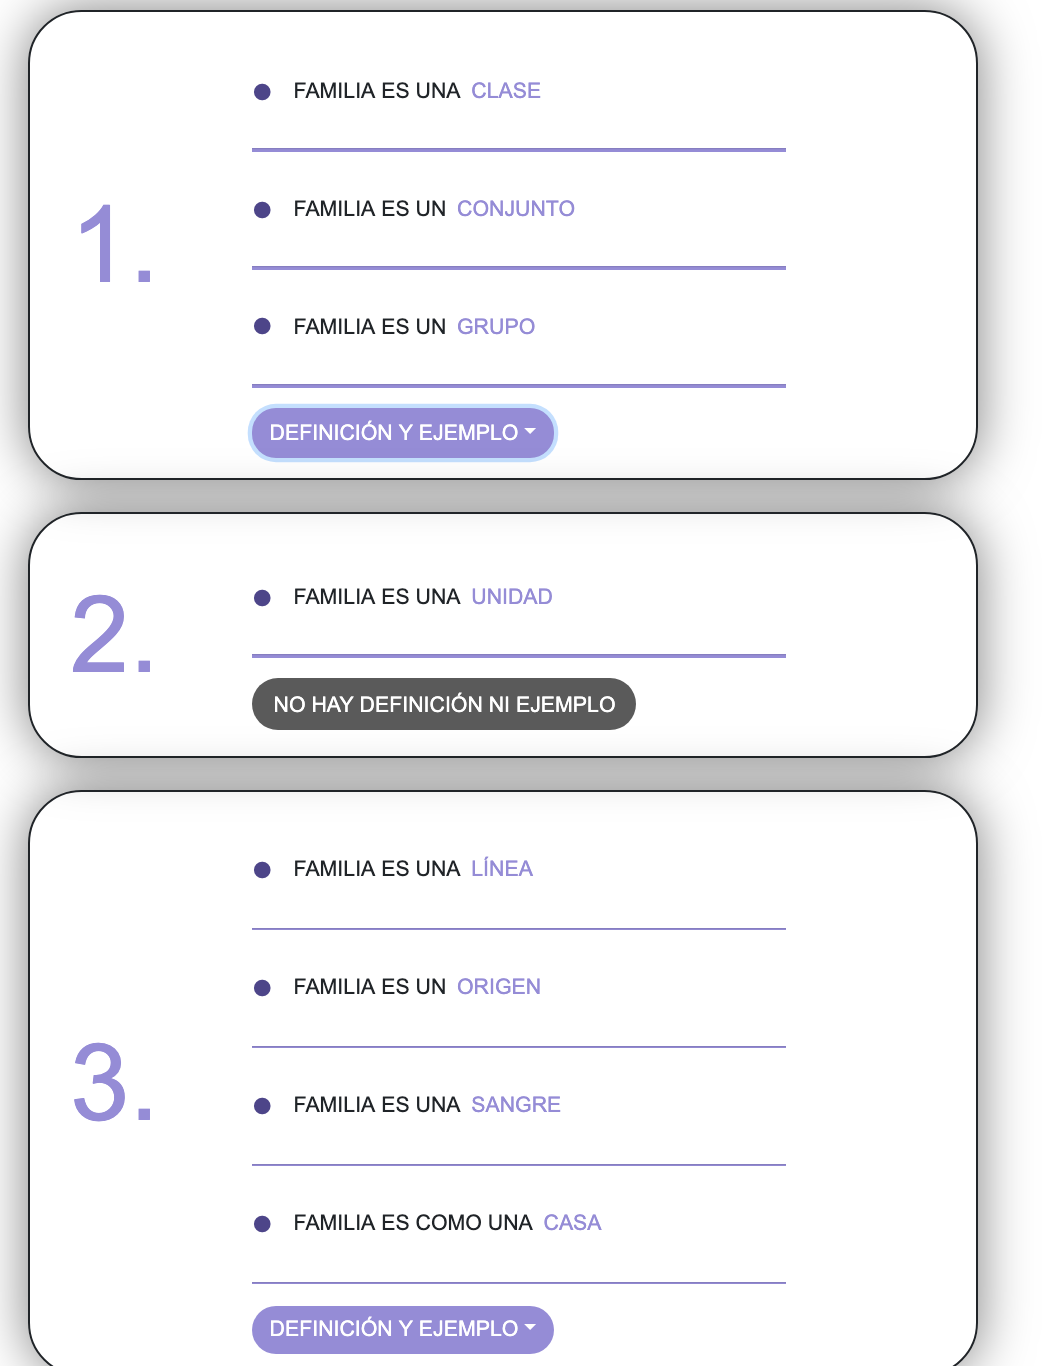
\includegraphics[width=.7\textwidth]{Imagenes/Bitmap/Capitulo4/EvaluacionFinal/10familiamayusculas.png}
	\centering
	\caption{Resultado obtenido para la palabra ``Familia'' convirtiendo el texto a mayúsculas}
	\label{fig:familiaMayusculas}
\end{figure}

\end{itemize}


Por último, se llevo a cabo la sección de uso libre, donde los alumnos nos decían palabras para buscar y posteriormente nos daban su opinión sobre los resultados. Las palabras introducidas fueron las siguientes:
\begin{itemize}
	\item La primera palabra que dijeron fue ``PASADO'' con un nivel de búsqueda fácil. Los resultados obtenidos se pueden ver en la Figura \ref{fig:pasadoFacil}. Los alumnos nos explicaron que los resultados obtenidos los entendían perfectamente.
	\begin{figure}[!h]
		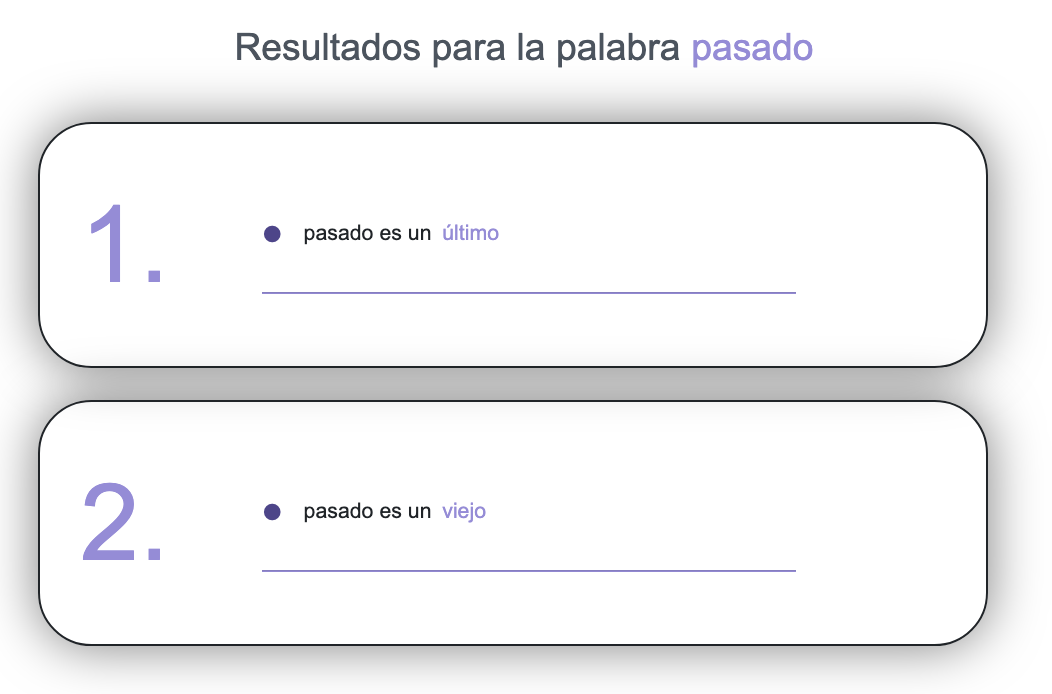
\includegraphics[width=.7\textwidth]{Imagenes/Bitmap/Capitulo4/EvaluacionFinal/1pasadofacil.png}
		\centering
		\caption{Resultado obtenido para la palabra ``Pasado'' con un nivel de búsqueda fácil}
		\label{fig:pasadoFacil}
	\end{figure}

	\item La siguiente palabra que dijeron fue ``ENAMORARSE'' con un nivel de búsqueda fácil. No mostraba ningún resultado puesto que es un verbo conjugado y en la aplicación solo se pueden introducir infinitivos, por lo que se buscó ``ENAMORAR'' con un nivel de búsqueda avanzado y añadiendo la opción de mostrar pictogramas. El resultado obtenido se puede ver en la Figura \ref{fig:enamorarAvanzado} y gracias al pictograma en el resultado ``atraer'' pudieron comprender su significado sin necesidad de explicárselo.
	\begin{figure}[!h]
		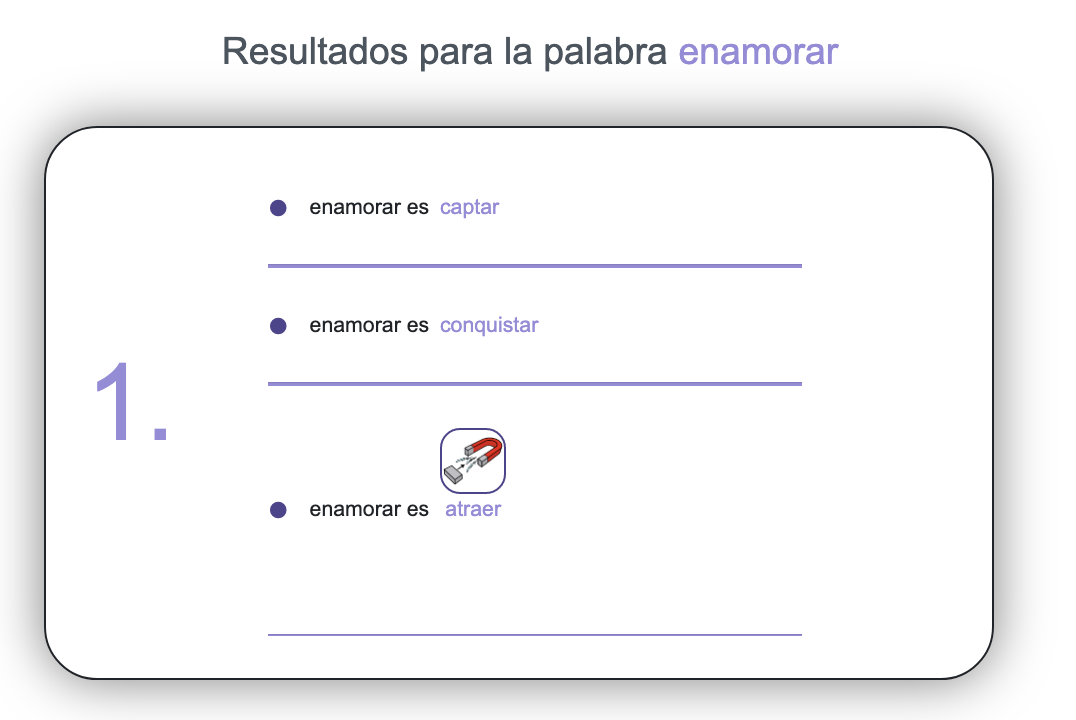
\includegraphics[width=.7\textwidth]{Imagenes/Bitmap/Capitulo4/EvaluacionFinal/2enamoraravanzado.png}
		\centering
		\caption{Resultado obtenido para la palabra ``Enamorar'' con un nivel de búsqueda avanzado y añadiendo pictogramas}
		\label{fig:enamorarAvanzado}
	\end{figure}

	\item Otra palabra que se buscó fue ``FIESTA'' con un nivel de búsqueda avanzado añadiendo la opción de mostrar definición y ejemplo. Los resultados obtenidos se pueden ver en la Figura \ref{fig:fiestaAvanzado}. En la ficha número 4 aparece la palabra ``suceso'', la cual a los alumnos les confunde un poco.
	Por ello, decidimos comprobar si la definición y el ejemplo que aparecía les podría ayudar (\textit{``Una ocasión en la que la gente puede reunirse para la interacción y el entretenimiento social'', ``Un evento social especificado vagamente'', ``Él planeo una fiesta para celebrar el Día de la Bastilla''}), pero esta definiciones y ejemplo llevan a un mayor grado de confusión al utilizar palabras como ``interacción'', ``vagamente'' o ``Día de la Bastilla'', términos con los cuales no están familiarizados y no conocen sus significados. En cambio, la definición que se muestra en la ficha número 2 (\textit{``Cualquier tipo de diversión que produce alegría''}), la entendían perfectamente al utilizar palabras que conocen su significado.
	\begin{figure}[!h]
		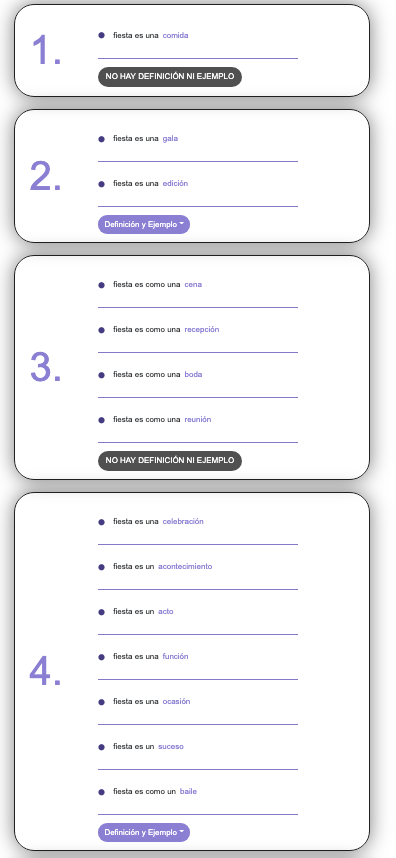
\includegraphics[width=.7\textwidth]{Imagenes/Bitmap/Capitulo4/EvaluacionFinal/3fiestaavanzadodef.png}
		\centering
		\caption{Resultado obtenido para la palabra ``Fiesta'' con un nivel de búsqueda avanzado y añadiendo tanto pictogramas como definición y ejemplo}
		\label{fig:fiestaAvanzado}
	\end{figure}

	\item A continuación, se introdujo la palabra  ``DETECTIVE'' con un nivel de búsqueda avanzado sin mostrar pictogramas ni definición y ejemplo. Los resultados obtenidos se pueden ver en la Figura \ref{fig:detectiveAvanzado}. El resultado de la primera ficha (``Detective es como un agente'') la entendían sin ningún problema, pero en la segunda ficha aparece el resultado ``Detective es un paco'', el cual hace referencia a una obra de teatro y los alumnos no entienden la relación existente entre ese término y el buscado.
	De los resultados obtenidos, se pinchó en uno de ellos para realizar la búsqueda de ese término en concreto en vez de tener que introducirlo en el buscador. La palabra pinchada fue ``investigador'' y de los resultados obtenidos, los alumnos entendieron todos los significados.
	\begin{figure}[!h]
		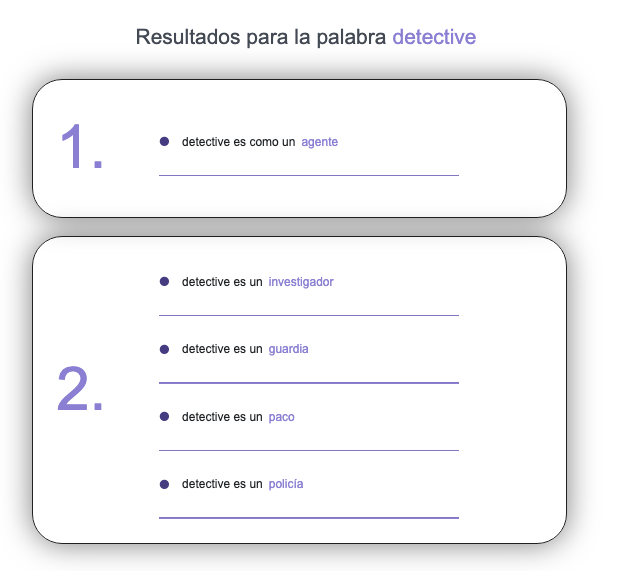
\includegraphics[width=.7\textwidth]{Imagenes/Bitmap/Capitulo4/EvaluacionFinal/4detectiveavanzado.png}
		\centering
		\caption{Resultado obtenido para la palabra ``Detective'' con un nivel de búsqueda avanzado}
		\label{fig:detectiveAvanzado}
	\end{figure}
	
	
	\item La siguiente palabra que se busco fue ``POLICIA'' con un nivel de búsqueda avanzado sin mostrar pictogramas ni definición y ejemplo. Los resultados obtenidos se pueden ver en la Figura \ref{fig:policiaAvanzado} y de la primera ficha sabían el significado de todos los conceptos excepto de ``dotación'' y de la segunda ficha no entendían la relación existente entre el concepto buscado y el resultado ``tira''. Posteriormente se les explicó que ``tira'' se refería al verbo tirar.
	\begin{figure}[!h]
		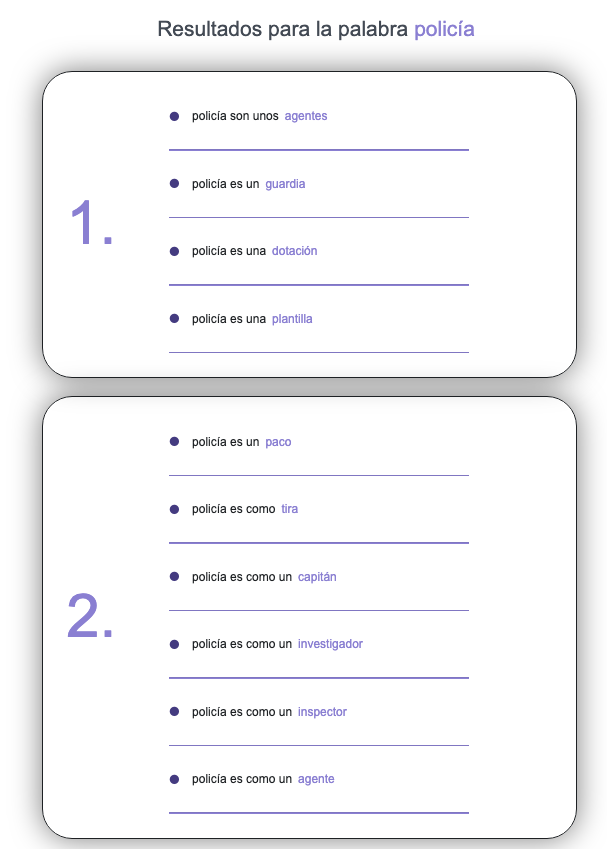
\includegraphics[width=.7\textwidth]{Imagenes/Bitmap/Capitulo4/EvaluacionFinal/5policiaavanzado.png}
		\centering
		\caption{Resultado obtenido para la palabra ``Policía'' con un nivel de búsqueda avanzado}
		\label{fig:policiaAvanzado}
	\end{figure}

 
 	\item Después se introdujo la palabra ``SIRENA'' con un nivel de búsqueda avanzado y mostrando pictogramas. Los resultados obtenidos se pueden ver en la Figura \ref{fig:sirenaAvanzado}, de los cuales entendían todos pero echaban en falta el resultado de sirena relacionado con el ser mitológico.
 \begin{figure}[!h]
 	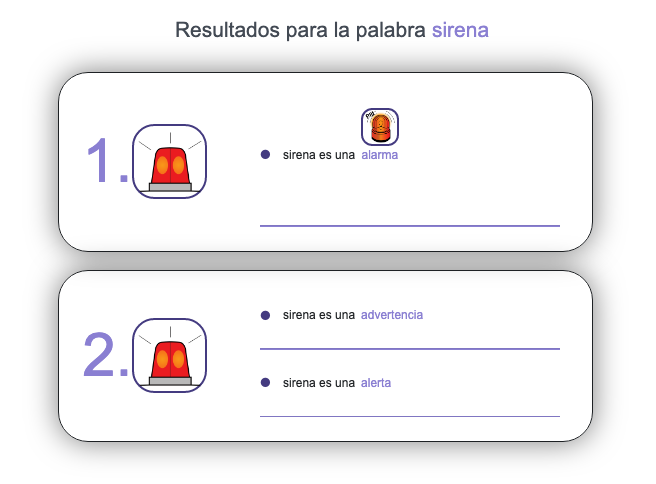
\includegraphics[width=.7\textwidth]{Imagenes/Bitmap/Capitulo4/EvaluacionFinal/6sirenaavanzado.png}
 	\centering
 	\caption{Resultado obtenido para la palabra ``Sirena'' con un nivel de búsqueda avanzado y añadiendo la opción de mostrar pictogramas}
 	\label{fig:sirenaAvanzado}
 \end{figure}
 
	\item Por último, se introdujo la palabra ``SOSO'' con un nivel de búsqueda avanzado y mostrando pictogramas. Los resultados obtenidos se pueden ver en la Figura \ref{fig:sosoAvanzado}, y fue correcto excepto que el pictograma de ``pesado'' en el cual aparece comida, no tiene relación directa con el propio significado de la palabra buscada.
\begin{figure}[!h]
	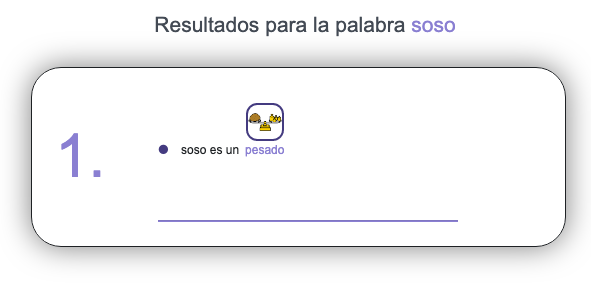
\includegraphics[width=.7\textwidth]{Imagenes/Bitmap/Capitulo4/EvaluacionFinal/7sosoavanzado.png}
	\centering
	\caption{Resultado obtenido para la palabra ``Soso'' con un nivel de búsqueda avanzado y añadiendo la opción de mostrar pictogramas}
	\label{fig:sosoAvanzado}
\end{figure}
	\end{itemize}


Después de realizar la evaluación guiada, les hicimos unas preguntas relacionadas con la usabilidad de la aplicación. Les preguntamos si la utilizarían habitualmente en su día a día y todos nos contestaron que sí, argumentando que les sirve para poder explicar y entender conceptos más complejos. Otra pregunta que se les realizó fue que si las opciones de mostrar o no tanto los pictogramas, como la definición y el ejemplo y convertir a mayúsculas o minúsculas preferían que fuese configurable o no. La respuesta de todos ellos es que es mucho más cómodo que sea configurable para que de esta forma pueden elegir como mostrar los resultados del concepto buscado.
También se les preguntó si les gustaba el color de la aplicación y si les había resultado fácil utilizarla, a lo que ellos nos contestaron que si a ambas preguntas.
Por último, se les preguntó si preferían los pictogramas a color o en blanco y negro y nos comentaron que a color por que son los que más familiarizados están y se comprenden mejor.
En definitiva, a todos los allí presentes les encantó la aplicación así como su funcionalidad.

Tras terminar la evaluación con el primer grupo, se realizó con el segundo grupo. En esta evaluación, se intentó seguir el mismo proceso utilizado con el primer grupo pero debido a que los alumnos eran más pequeños y se desconcentraban con mayor facilidad, solo pudimos seguir la parte guiada en unas cuantas preguntas y el resto se analizó con el profesor en ese momento presente. Los resultados obtenidos se explican a continuación:

\begin{itemize}
	\item PRUEBA 1 - Búsqueda con nivel fácil: La primera palabra introducida fue ``PUENTE'' con un nivel de búsqueda fácil y con las opciones de pictograma y definición y ejemplo predeterminadas. En la Figura \ref{fig:puenteFacil} se pueden ver los resultados obtenidos, donde a los alumnos no les quedaba claro los distintos significados, asi que probamos a añadir la opción de mostrar pictogramas y de esta forma si los comprendían.
	
	\item PRUEBA 2 - Búsqueda con nivel medio: Se introdujo la misma palabra ``PUENTE'' pero aumentando el nivel de búsqueda a medio. En la Figura \ref{fig:puenteMedio} se pueden ver los resultados obtenidos. En este caso hubo ocurrió lo mismo que en la prueba 1, y es que si se añaden los pictogramas entienden mucho mejor los resultados que sin ellos, por ejemplo para la palabra ``arco''.
	
	\item PRUEBA 3 - Búsqueda con nivel avanzado: Esta vez, se volvió a introducir la palabra ``PUENTE'' con un nivel de búsqueda avanzado. En la Figura  \ref{fig:puenteAvanzado} se pueden ver los resultados obtenidos donde se puede ver que con este nivel se muestra un resultado más que en el anterior nivel. A los alumnos les ocurrió lo mismo que al grupo 1 con la palabra ``placa'', ya que no entendían su significado en dicho contexto.
	
	\item PRUEBA 4 - Obteniendo un único resultado: La palabra introducida fue ``DICTADOR'' con un nivel de búsqueda avanzado y sin mostrar ni pictogramas ni definición y ejemplo. En la Figura \ref{fig:dictadorAvanzado} se pueden ver los resultados obtenidos, de estos no entendían el significado de la palabra ``soberano'', asi que se modificó el nivel a medio donde comprendían mejor los resultados. En general, ellos entendían la palabra ``dictador'' como persona que dicta un texto a alguien, por lo que a través de la aplicación supieron nuevas acepciones para dicho  concepto.

	\item PRUEBA 5 - Obteniendo varios resultados (I):  Se introdujo la palabra ``DEFENSA'' con un nivel de búsqueda fácil. En la Figura \ref{fig:defensaFacil} se pueden ver los resultados obtenidos. Estos resultados eran bastante complicados de entender para los alumnos. En la dicha número 1, les confundía la palabra ``construcción'', aunque explicándoselo si sabían lo que era.
	
	\item PRUEBA 6 - Obteniendo varios resultados (II):  Se realizó otra prueba para obtener varios resultados. En este caso de introdujo la palabra ``DANZA''  sin pictogramas y con un nivel de búsqueda avanzado. En la Figura \ref{fig:danzaAvanzado} se pueden ver los resultados obtenidos, de los cuales los alumnos entendieron todos sin ningún problema.
	
	\item PRUEBA 7 - Obtención de metáforas:  Se introdujo la palabra ``PORTERO'' con un nivel de búsqueda avanzado y añadiendo la opción de mostrar pictogramas. Se puede ver en la Figura \ref{fig:porteroAvanzado} los resultados obtenidos. Los alumnos conocían los significados que están relacionados con portero de deporte y portero de profesión, pero la palabra ``funcionario'' y ``administrador'' no la entendían. A parte, echaban en falta que apareciese el resultado de portero automático.
\end{itemize}


A partir de este momento, la prueba se realizó con el profesor. Nos comentó que en su día a día al impartir clase existían ciertas palabras que no sabe como explicar su significado a los alumnos.
Una de ellas fue ``TALAR'', la cuál la buscamos en la aplicación con nivel de búsqueda avanzado y añadiendo pictogramas. El resultado obtenido se puede ver en la Figura \ref{fig:talarAvanzado} y este era correcto, pero nos comentó que faltaba el pictograma que representa el concepto en sí. Del resultado que se obtuvo (``talar es cortar''), el pictograma de ``cortar'' no era el adecuado según su acepción, ya que debería aparecer uno de ``talar'' en vez de ``cortar''.

\begin{figure}[!h]
	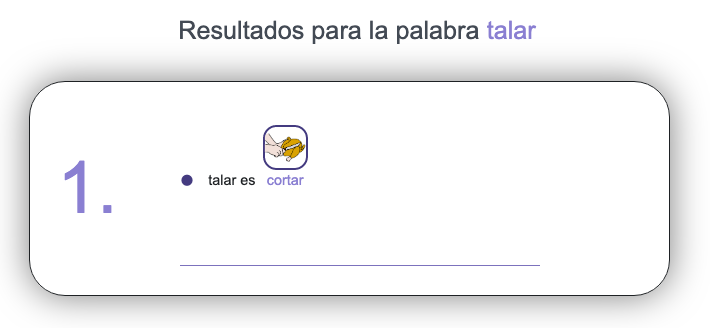
\includegraphics[width=.7\textwidth]{Imagenes/Bitmap/Capitulo4/EvaluacionFinal/talaravanzado.png}
	\centering
	\caption{Resultado obtenido para la palabra ``Talar'' con un nivel de búsqueda avanzado y añadiendo la opción de mostrar pictogramas}
	\label{fig:talarAvanzado}
\end{figure}

Otra palabra que se buscó fue ``SACUDIR'' con nivel de búsqueda avanzado y mostrando tanto los pictogramas como la definición y el ejemplo. Los resultados obtenidos se pueden ver en la Figura \ref{fig:sacudirAvanzado} . Algunos de estos fueron correctos y otros no. De los correctos, el profesor indicó que debería aparecer primero el resultado más común o el que mejor define el concepto (en este caso ``mover'' antes que ``batir''), y otros resultados como ``trasladar'' y ``reducir'' no deberían aparecer por que no están relacionados con el concepto buscado.
Por otro lado, la definición y ejemplo que aparecen son correctos (\textit{Mover o causar movimiento de un lado a otro}). 
\begin{figure}[!h]
	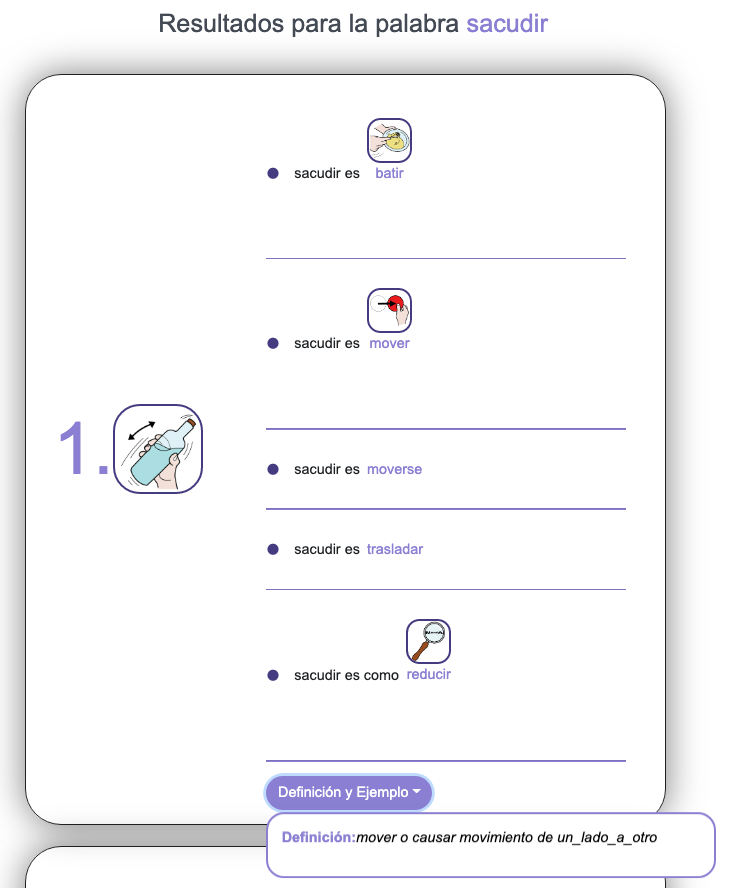
\includegraphics[width=.7\textwidth]{Imagenes/Bitmap/Capitulo4/EvaluacionFinal/sacudiravanzado.png}
	\centering
	\caption{Resultado obtenido para la palabra ``Sacudir'' con un nivel de búsqueda avanzado y añadiendo la opción de mostrar pictogramas y de definición y ejemplo}
	\label{fig:sacudirAvanzado}
\end{figure}

Nos comentó también que prefiere que la aplicación este en mayúsculas, pero que sea configurable. Y lo mismo para los pictogramas.

Finalmente tras realizar dicha evaluación con dos grupos tan dispares entre sí y con necesidades totalmente distintas, llegamos a la conclusión de que la aplicación solamente sería útil para usuarios cuyo grado de discapacidad no fuera muy elevado. Puesto que si la aplicación fuera destinada para personas como las del grupo 2 no les ayudaría, si no todo lo contrario, les complicaría aún más el poder entender el significado de cierto concepto.

Ellos necesitan resultados mucho más fáciles de los que la aplicación devuelve y organizados en una estructura totalmente distinta a la que nosotros implementamos. En cambio, para personas con un mayor grado de independencia les resultaría bastante útil y les simplificaría ciertas situaciones que puedan vivir.

